\documentclass[../DefinizioneDiProdotto_v3.0.0.tex]{subfiles}
\begin{document}

\section{Specifica dei componenti}

\subsection{\texttt{Front-End}}
		\begin{figure}[!h]
			\centering
			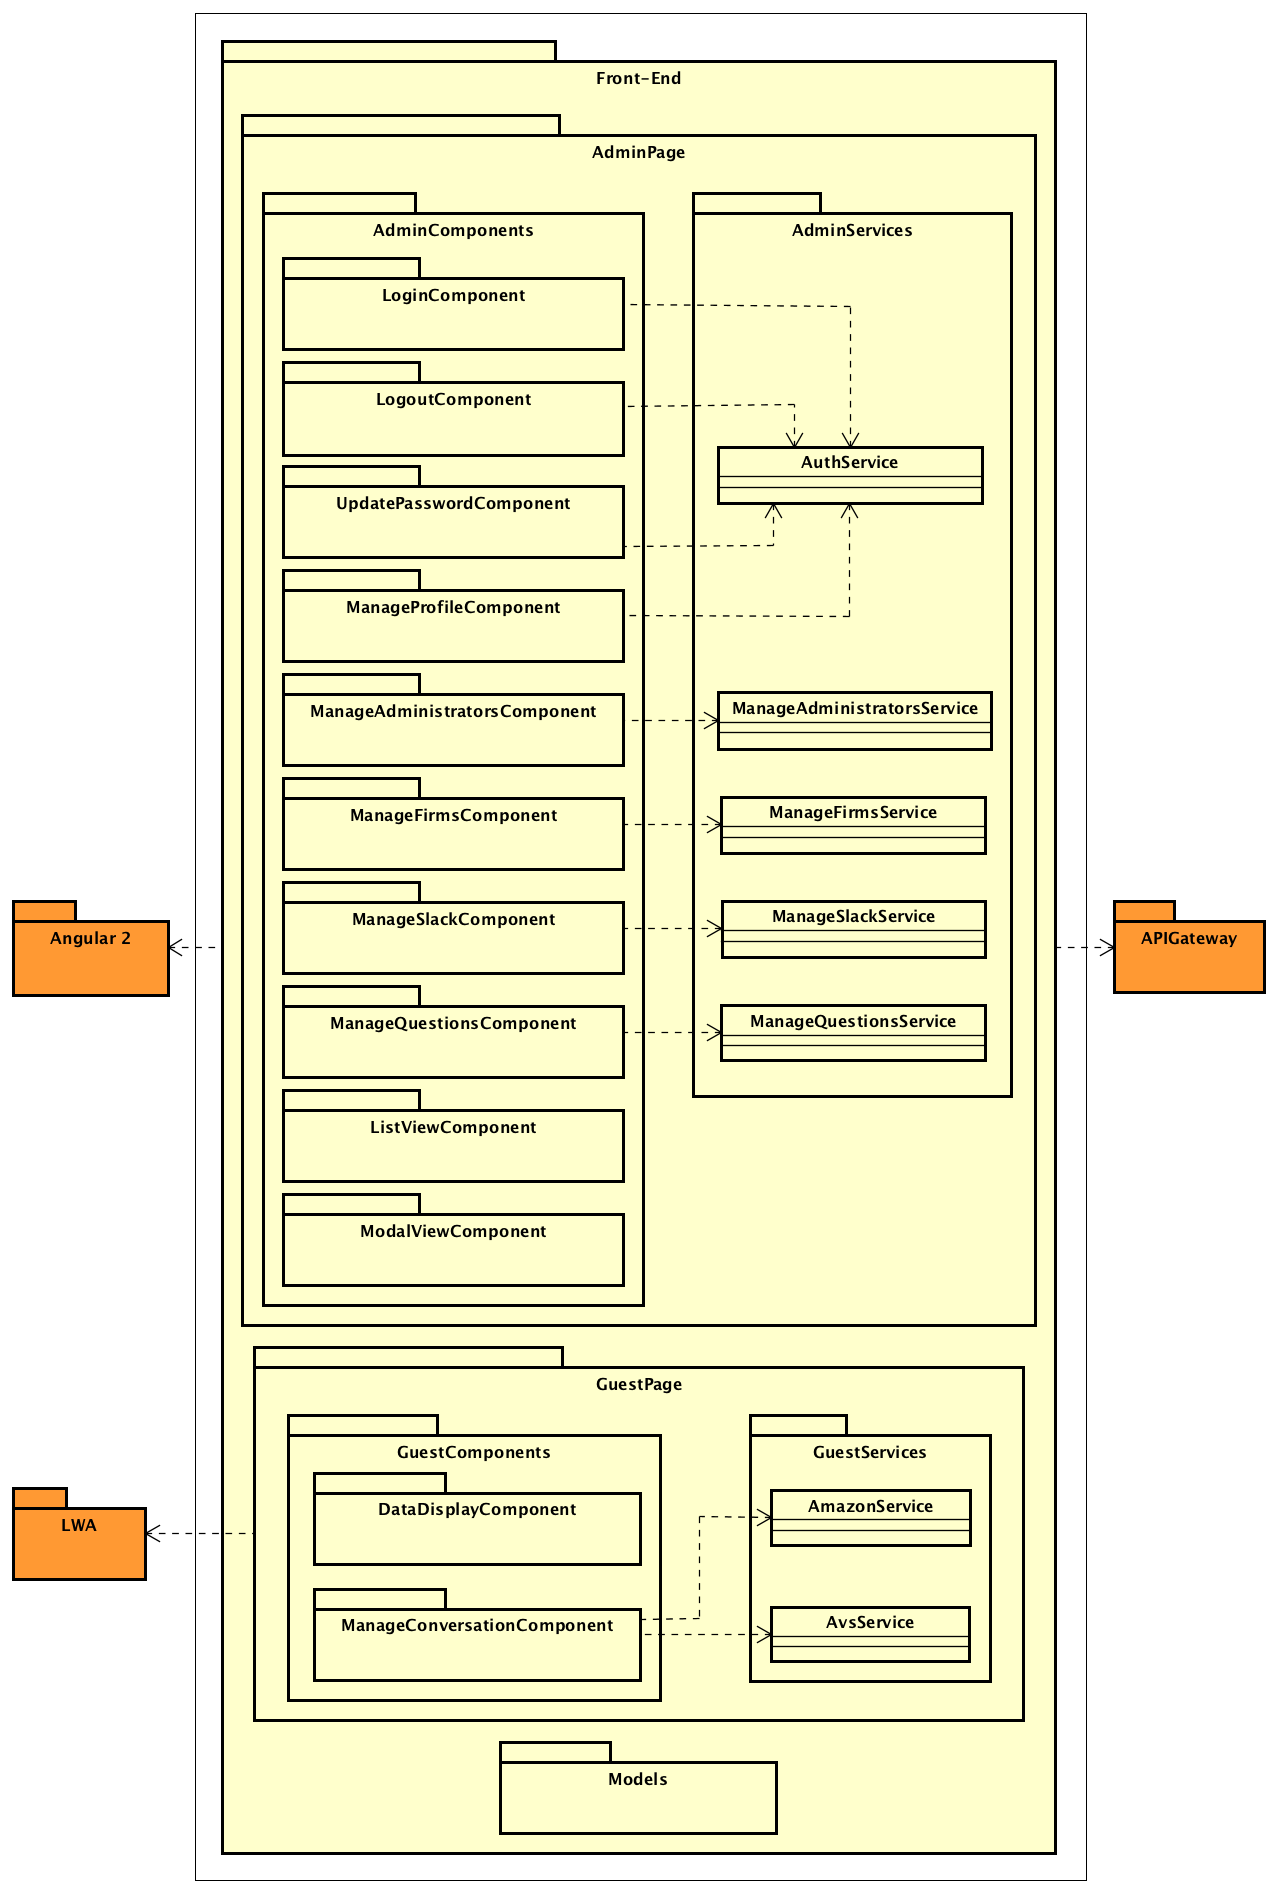
\includegraphics[scale=0.4]{Architettura/Front-end.png}
			\caption{Schema del componente \texttt{Front-End - Schema Generale}}
		\end{figure}
		\subparagraph{Descrizione}: Package che rappresenta il client dell'applicazione
		\subparagraph{Package contenuti}:
		\begin{itemize}
			\item Front-End :: AdminPage: Package dedicato alla parte client dell'Admin e del SuperAdmin;
			\item Front-End :: GuestPage: Package dedicato alla parte d'interfaccia client disponibile per l'ospite e per l'utente.
		\end{itemize}


	\clearpage
	\subsubsection{\texttt{Front-End :: AdminPage}}
	\begin{figure}[!h]
		\centering
		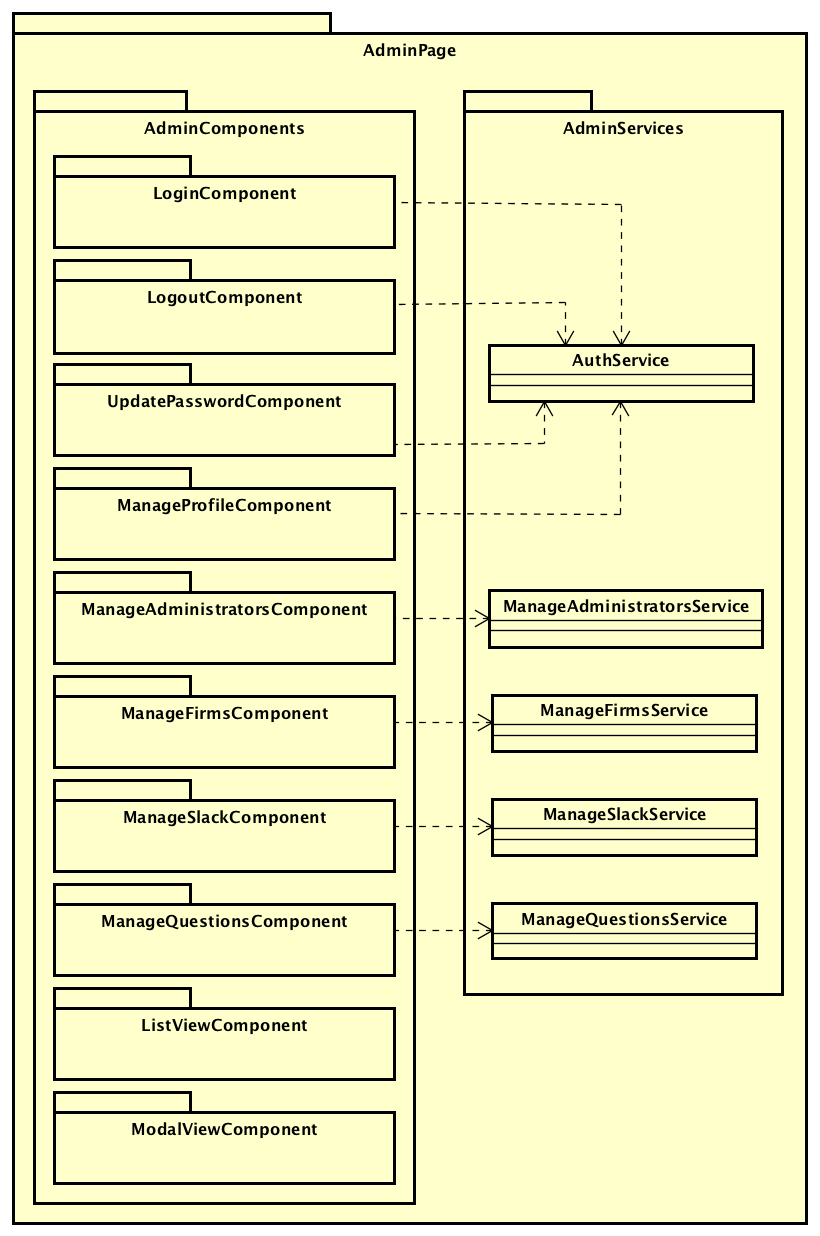
\includegraphics[scale=0.45]{Architettura/Front-End/AdminPage/AdminPage.png}
		\caption{Schema del componente \texttt{Front-End :: AdminPage}}
	\end{figure}
			\subparagraph{Descrizione}: Package dedicato alla parte client fruibile da un amministratore
			\subparagraph{Padre}: Front-End
			\subparagraph{Package contenuti}:
			\begin{itemize}
				\item AdminPage :: AdminComponents: Package contenente tutti i componenti necessari al Front-End della console amministrativa, comprensivi quindi dei models che andranno ad utilizzare e delle relative view e controller;
				\item AdminPage :: AdminServices: Package che fornisce tutti i servizi utilizzabili dai componenti presenti in AdminComponents.
			\end{itemize}

	\subsubsection{\texttt{Front-End :: AdminPage :: AdminComponents}}

		\subparagraph{Descrizione}: Classe contenente tutti i metodi necessari a gestire il Front-End della console amministrativa
		\subparagraph{Padre}: AdminPage
		\subparagraph{Package contenuti}:
		\begin{itemize}
			\item AdminPage :: AdminComponents :: LoginComponent: Componente che contiene al suo interno la sua view, il suo controller, ed i models di cui necessita
			\item AdminPage :: AdminComponents :: LogoutComponent: Componente che contiene al suo interno la sua view, il suo controller, ed i models di cui necessita
			\item AdminPage :: AdminComponents :: ManageAdministratorsComponent: Componente che contiene al suo interno la sua view, il suo controller, ed i models di cui necessita
			\item AdminPage :: AdminComponents :: ManageFirmsComponent: Componente che contiene al suo interno la sua view, il suo controller, ed i models di cui necessita
			\item AdminPage :: AdminComponents :: ManageProfileComponent: Componente che contiene al suo interno la sua view, il suo controller, ed i models di cui necessita
			\item AdminPage :: AdminComponents :: ManageQuestionsComponent: Componente che contiene al suo interno la sua view, il suo controller, ed i models di cui necessita
			\item AdminPage :: AdminComponents :: ManageSlackComponent: Componente che contiene al suo interno la sua view, il suo controller, ed i models di cui necessita
			\item AdminPage :: AdminComponents :: UpdatePasswordComponent: Componente che contiene al suo interno la sua view, il suo controller, ed i models di cui necessita
			\item AdminPage :: AdminComponents :: ListViewComponent: Componente che contiene al suo interno la sua view, il suo controller, ed i models di cui necessita
			\item AdminPage :: AdminComponents :: ModalViewComponent: Componente che contiene al suo interno la sua view, il suo controller, ed i models di cui necessita
		\end{itemize}

\newpage
	\subsubsection{\texttt{Front-End :: AdminPage :: AdminComponents :: LoginComponent}}
	\begin{figure}[!h]
		\centering
		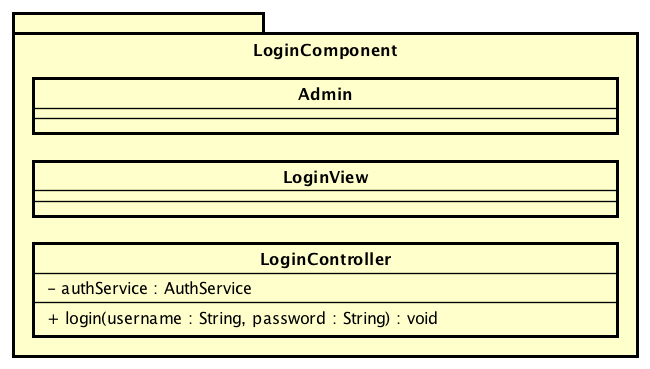
\includegraphics[scale=0.7]{Architettura/Front-End/AdminPage/AdminComponents/LoginComponent.png}
		\caption{Schema del componente \texttt{Front-End :: AdminPage :: AdminComponents :: LoginComponent}}
	\end{figure}
			\subparagraph{Descrizione}: Componente che contiene al suo interno la sua view, il suo controller, ed i models di cui necessita
			\subparagraph{Padre}: AdminComponents
			\paragraph{\texttt{Front-End :: AdminPage :: AdminComponents :: LoginComponent :: LoginController}}
				\subparagraph{Descrizione}: Controller che gestisce la view di LoginView permettendo ad un amministratore di effettuare l'accesso alla console amministrativa
				\subparagraph{Costanti}:
				\begin{itemize}
					\item \texttt{authService: AuthService}: Attributo che rappresenta una istanza del service AuthService e ne mette a disposizione i metodi.
				\end{itemize}
				\subparagraph{Metodi}:
				\begin{itemize}
					\item \texttt{login}:
					\subparagraph{Descrizione}:Funzione che permette all'amministratore di effettuare l'accesso alla console amministrativa
					\subparagraph{Argomenti}:
					\begin{itemize}
						\item \texttt{email : string}: Parametro che indica la email inserita dall'amministratore.
						\item \texttt{password : string}: Parametro che indica la password inserita dall'amministratore.
					\end{itemize}
				\end{itemize}\vspace{0.5em}
	  		\paragraph{\texttt{Front-End :: AdminPage :: AdminComponents :: LoginComponent :: LoginView}}
				\subparagraph{Descrizione}: View di Login, permette ad un amministratore di effettuare l'accesso alla console amministrativa
				\subparagraph{Utilizzo}: View di Login
\newpage
	\subsubsection{\texttt{Front-End :: AdminPage :: AdminComponents :: LogoutComponent}}
	\begin{figure}[!h]
		\centering
		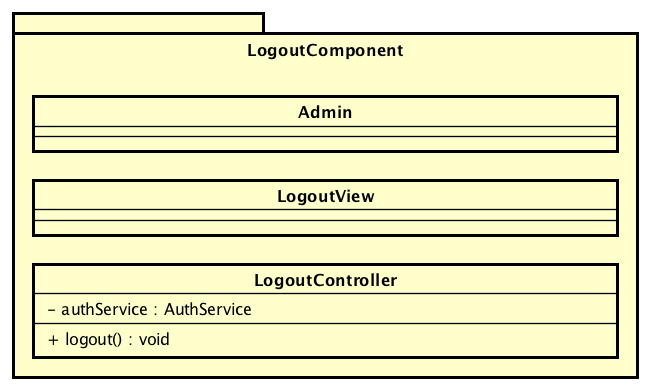
\includegraphics[scale=0.7]{Architettura/Front-End/AdminPage/AdminComponents/LogoutComponent.png}
		\caption{Schema del componente \texttt{Front-End :: AdminPage :: AdminComponents :: LogoutComponent}}
	\end{figure}

			\subparagraph{Descrizione}: Componente che contiene al suo interno la sua view, il suo controller, ed i models di cui necessita
			\subparagraph{Padre}: AdminComponents
	  		\paragraph{\texttt{Front-End :: AdminPage :: AdminComponents :: LogoutComponent :: LogoutController}}
				\subparagraph{Descrizione}: Componente dedicato all'operazione di logout
				\subparagraph{Costanti}:
				\begin{itemize}
					\item \texttt{authService: AuthService}: Attributo che rappresenta una istanza del service AuthService e ne mette a disposizione i metodi.
				\end{itemize}
				\subparagraph{Metodi}:
				\begin{itemize}
					\item \texttt{logout}: Funzione che permette ad un amministratore correttamente loggato nell'area amministrativa di effettuare il logout e terminare la sessione
				\end{itemize}\vspace{0.5em}
			\paragraph{\texttt{Front-End :: AdminPage :: AdminComponents :: LogoutComponent :: LogoutView}}
				\subparagraph{Descrizione}: View del componente dedicato all'operazione di logout

	\newpage
	\subsubsection{\texttt{Front-End :: AdminPage :: AdminComponents :: ManageAdministratorsComponent}}
	\begin{figure}[!h]
		\centering
		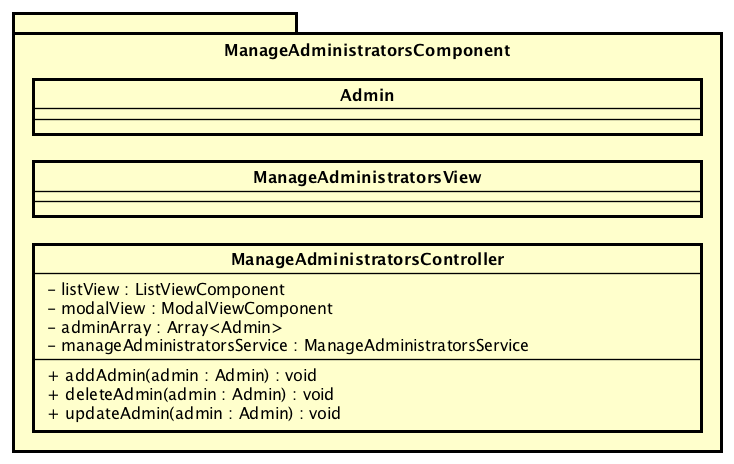
\includegraphics[scale=0.7]{Architettura/Front-End/AdminPage/AdminComponents/ManageAdministratorsComponent.png}
		\caption{Schema del componente \texttt{Front-End :: AdminPage :: AdminComponents :: ManageAdministratorsComponent}}
	\end{figure}

			\subparagraph{Descrizione}: Componente che contiene al suo interno la sua view, il suo controller, ed i models di cui necessita
			\subparagraph{Padre}: AdminComponents
				\paragraph{\texttt{Front-End :: AdminPage :: AdminComponents :: ManageAdministratorsComponent :: ManageAdministratorsController}}
		      		\subparagraph{Descrizione}: Controller che gestisce la view di ManageAdministrators permettendo ad un SuperAdmin di gestire le informazioni degli altri amministratori
			      	\subparagraph{Attributi}:
					\begin{itemize}
						\item \texttt{listView: ListView}: Attributo che indica la lista che andrà a contenere gli amministratori.
						\item \texttt{modalView: ModalView}: Attributo che indica il model che conterrà la form per aggiungere o aggiornare un amministratore.
						\item \texttt{adminArray: AdminArray}: Attributo che indica gli amministratori presenti nel sistema.
						\item \texttt{manageAdministratorsService: ManageAdministratorsService}: Attributo che rappresenta una istanza del service ManageAdministratorsService e ne mette a disposizione i metodi.
					\end{itemize}
			      	\subparagraph{Metodi}:
					\begin{itemize}
						\item \texttt{addAdmin}
						\subparagraph{Descrizione}:Funzione che permette ad un SuperAdmin di aggiungere un nuovo amministratore al sistema
						\subparagraph{Argomenti}:
						\begin{itemize}
							\item \texttt{admin : Admin}: Parametro che indica l'amministratore da aggiungere.
						\end{itemize}

						\item \texttt{deleteAdmin}
						\subparagraph{Descrizione}:Funzione che permette ad un SuperAdmin di eliminare un Admin dal sistema
						\subparagraph{Argomenti}:
						\begin{itemize}
							\item \texttt{admin : Admin}: Parametro che indica l'amministratore da rimuovere.
						\end{itemize}
						\item \texttt{updateAdmin}:
						\subparagraph{Descrizione}:Funzione che permette ad un SuperAdmin di modificare la password di un Admin presente nel sistema
						\subparagraph{Argomenti}:
						\begin{itemize}
							\item \texttt{admin : Admin}: Parametro che indica l'amministratore da aggiornare.
						\end{itemize}
					\end{itemize}
				\paragraph{\texttt{Front-End :: AdminPage :: AdminComponents :: ManageAdministratorsComponent :: ManageAdministratorsView}}
					\subparagraph{Descrizione}: View di ManageAdministrators, permette ad un SuperAdmin di gestire le informazioni degli altri amministratori
					\subparagraph{Utilizzo}: View di ManageAdministrators

	\newpage
	\subsubsection{\texttt{Front-End :: AdminPage :: AdminComponents :: ManageFirmsComponent}}
	\begin{figure}[!h]
		\centering
		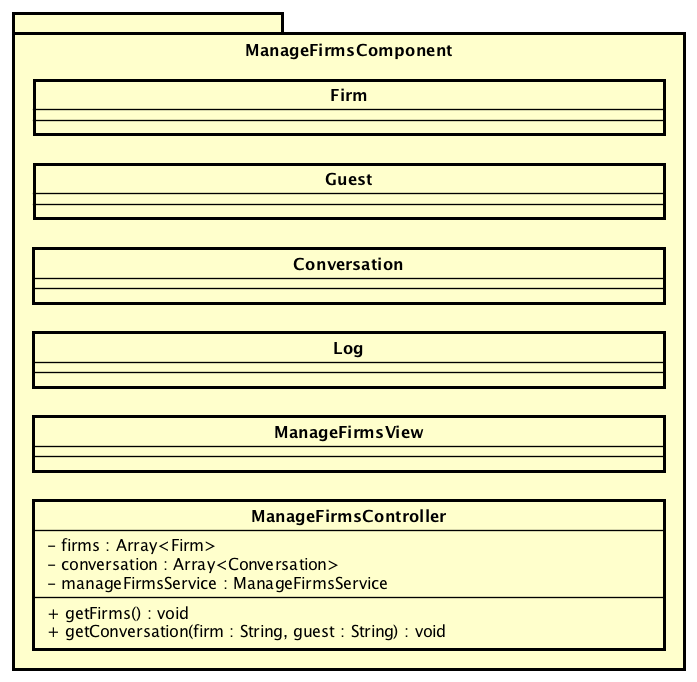
\includegraphics[scale=0.7]{Architettura/Front-End/AdminPage/AdminComponents/ManageFirmsComponent.png}
		\caption{Schema del componente \texttt{Front-End :: AdminPage :: AdminComponents :: ManageFirmsComponent}}
	\end{figure}

			\subparagraph{Descrizione}: Componente che contiene al suo interno la sua view, il suo controller, ed i models di cui necessita
			\subparagraph{Padre}: AdminComponents
				\paragraph{\texttt{Front-End :: AdminPage :: AdminComponents :: ManageFirmsComponent :: ManageFirmsController}}
					\subparagraph{Descrizione}: Componente utilizzato per la gestione degli oggetti di tipo Firm
					\subparagraph{Attributi}:
					\begin{itemize}
						\item \texttt{firms: Array<Firm>}: Attributo che indica le aziende presenti nel sistema.
						\item \texttt{manageFirmsService: ManageFirmsService}: Attributo che rappresenta una istanza del service ManageFirmsService e ne mette a disposizione i metodi.
					\end{itemize}
					\subparagraph{Metodi}:
					\begin{itemize}
						\item \texttt{getFirms}:
							\subparagraph{Descrizione}: Funzione che ottiene tutte le aziende presenti nel sistema
						\item \texttt{getConversation}:
						\subparagraph{Descrizione}: Funzione che ottiene tutte le conversazioni di un utente di una azienda presenti nel sistema
						\subparagraph{Argomenti}:
						\begin{itemize}
							\item \texttt{firm : string}: Parametro che indica il nome dell'azienda.
							\item \texttt{guest : string}: Parametro che indica il nome dell'ospite.
						\end{itemize}
					\end{itemize}

				\paragraph{\texttt{Front-End :: AdminPage :: AdminComponents :: ManageFirmsComponent :: ManageFirmsView}}
					\subparagraph{Descrizione}: View utilizzata per la scelta degli oggetti di tipo Firm


	\newpage
	\subsubsection{\texttt{Front-End :: AdminPage :: AdminComponents :: ManageProfileComponent}}
	\begin{figure}[!h]
		\centering
		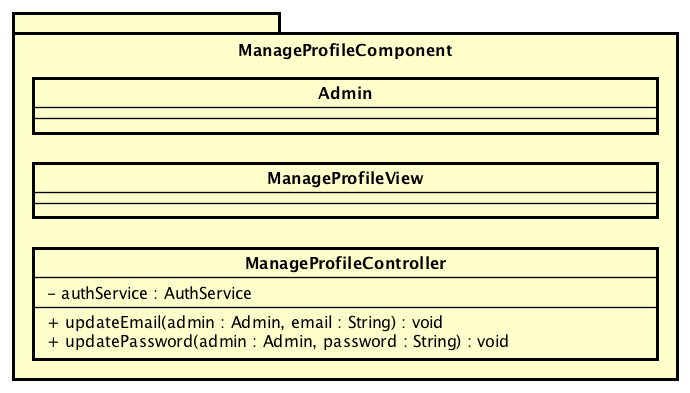
\includegraphics[scale=0.7]{Architettura/Front-End/AdminPage/AdminComponents/ManageProfileComponent.png}
		\caption{Schema del componente \texttt{Front-End :: AdminPage :: AdminComponents :: ManageProfileComponent}}
	\end{figure}
			\subparagraph{Descrizione}: Componente che contiene al suo interno la sua view, il suo controller, ed i models di cui necessita
			\subparagraph{Padre}: AdminComponents
				\paragraph{\texttt{Front-End :: AdminPage :: AdminComponents :: ManageProfileComponent :: ManageProfileView}}
					\subparagraph{Descrizione}: View di ManageProfile, permette ad un amministratore di gestire il proprio profilo nell'area amministrativa
				\paragraph{\texttt{Front-End :: AdminPage :: AdminComponents :: ManageProfileComponent :: ManageProfileController}}

					\subparagraph{Descrizione}: Controller che gestisce la view di ManageProfileView permettendo ad un amministratore di gestire il proprio profilo nell'area amministrativa
					\subparagraph{Attributi}:
					\begin{itemize}
						\item \texttt{authService: AuthService}: Attributo che rappresenta una istanza del service AuthService e ne mette a disposizione i metodi.
					\end{itemize}
					\subparagraph{Metodi}:
					\begin{itemize}
						\item \texttt{updateEmail}:
						\subparagraph{Descrizione}: Funzione che permette ad un amministratore di aggiornare la propria email
						\subparagraph{Argomenti}:
						\begin{itemize}
							\item \texttt{admin : Admin}: Parametro che indica l'amministratore corrente.
							\item \texttt{email : string}: Parametro che indica la nuova email inserita dall'amministratore.
						\end{itemize}
						\item \texttt{updatePassword}:
						\subparagraph{Descrizione}:Funzione che permette ad un amministratore di aggiornare la propria password
						\subparagraph{Argomenti}:
						\begin{itemize}
							\item \texttt{admin : Admin}: Parametro che indica l'amministratore corrente.
							\item \texttt{password : string}: Parametro che indica la nuova password inserita dall'amministratore.
						\end{itemize}
					\end{itemize}\vspace{0.5em}
				\paragraph{\texttt{Front-End :: AdminPage :: AdminComponents :: ManageProfileComponent :: ManageProfileView}}

					\subparagraph{Descrizione}: View di ManageProfile, permette ad un amministratore di gestire il proprio profilo nell'area amministrativa


	\newpage
	\subsubsection{\texttt{Front-End :: AdminPage :: AdminComponents :: ManageQuestionsComponent}}
	\begin{figure}[!h]
		\centering
		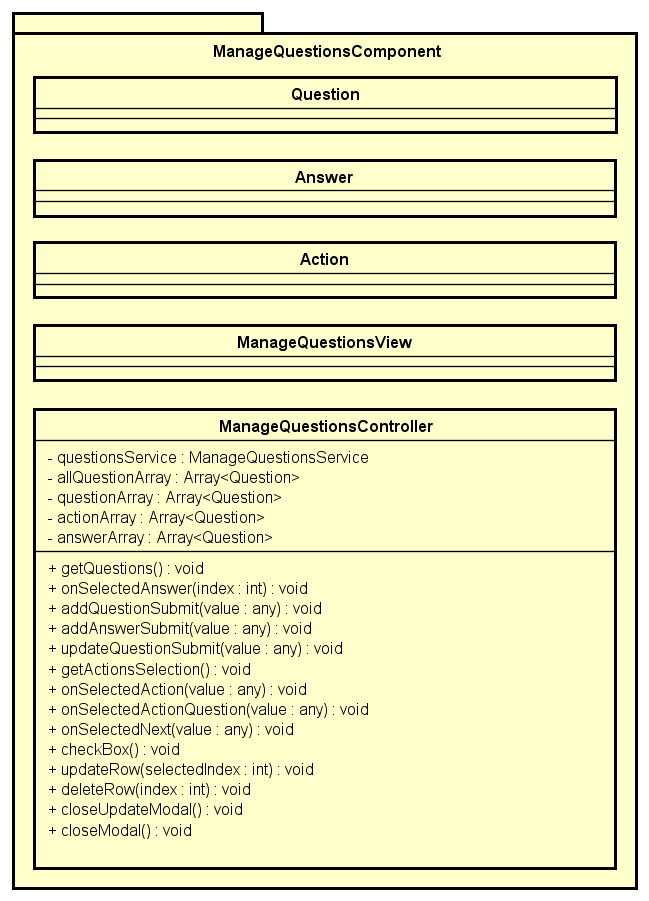
\includegraphics[scale=0.7]{Architettura/Front-End/AdminPage/AdminComponents/ManageQuestionsComponent.png}
		\caption{Schema del componente \texttt{Front-End :: AdminPage :: AdminComponents :: ManageQuestionsComponent}}
	\end{figure}
			\subparagraph{Descrizione}: Componente che contiene al suo interno la sua view, il suo controller, ed i models di cui necessita
			\subparagraph{Padre}: AdminComponents
			      \paragraph{\texttt{Front-End :: AdminPage :: AdminComponents :: ManageQuestionsComponent :: ManageQuestionsController}}
			      	\subparagraph{Descrizione}: Componente per le domande e interazioni
			      	\subparagraph{Utilizzo}: Componente utilizzato per le domande e interazioni
			      	\subparagraph{Attributi}:
      	      			\begin{itemize}
							\item \texttt{manageQuestionsService : ManageQuestionsService}: Attributo che rappresenta una istanza del service ManageQuestionsService e ne mette a disposizione i metodi.
							\item \texttt{allQuestionArray: Array<Question}: Parametro che indica la lista delle domande presenti nel sistema comprensive delle proprie risposte selezionate.
							\item \texttt{questionsArray: Array<Question}: Parametro che indica la lista delle domande presenti nel sistema comprensive delle proprie risposte.
							\item \texttt{actionArray: Array<Action>}: Parametro che indica la lista delle action presenti nel sistema.
							\item \texttt{answerArray: Array<Answer>}: Parametro che indica la lista delle risposte presenti nel sistema.

						\end{itemize}
						\subparagraph{Metodi}:
						\begin{itemize}
							\item \texttt{getQuestions}:
							\subparagraph{Descrizione}:Funzione che permette di ottenere la lista delle domande presenti nel sistema

							\item \texttt{onSelectedAnswer}:
							\subparagraph{Descrizione}:Funzione che permette di selezionare una domanda.
							\subparagraph{Argomenti}:
							\begin{itemize}
								\item \texttt{index : int}: Parametro che indica l'indice.
							\end{itemize}
							
							\item \texttt{addQuestionSubmit}:
							\subparagraph{Descrizione}:Funzione che permette di aggiungere una question.
							\subparagraph{Argomenti}:
							\begin{itemize}
								\item \texttt{value:any}: Parametro che indica la question.
							\end{itemize}					
														
							\item \texttt{addAnswerSubmit}:
							\subparagraph{Descrizione}:Funzione che permette di aggiungere un'answer ad una question.
							\subparagraph{Argomenti}:
							\begin{itemize}
								\item \texttt{value:any}: Parametro che indica l'answer da aggiungere' .
							\end{itemize}
							
							\item \texttt{updateQuestionSubmit}:
							\subparagraph{Descrizione}:Funzione che permette di modificare una question.
							\subparagraph{Argomenti}:
							\begin{itemize}
								\item \texttt{value:any}: Parametro che contiene la question da modificare.
							\end{itemize}

							\item \texttt{getActionsSelection}:
							\subparagraph{Descrizione}:Funzione che permette di ricavare le action da inserire nella select, diviso nei due vettori, questionAction e Actions.


							\item \texttt{onSelectedAction}:
							\subparagraph{Descrizione}:Funzione che permette di aggiungere un'action perchè selezionata.
							\subparagraph{Argomenti}:
							\begin{itemize}
								\item \texttt{value:any}: Parametro che indica l'action.
							\end{itemize}

							\item \texttt{onSelectedActionQuestion}:
							\subparagraph{Descrizione}:Funzione che permette di aggiungere una questionAction.
							\subparagraph{Argomenti}:
							\begin{itemize}
								\item \texttt{value:any}: Parametro che indica l'action.
							\end{itemize}

							\item \texttt{onSelectedNext}:
							\subparagraph{Descrizione}:Funzione che permette di aggiungere la prossima domanda.
							\subparagraph{Argomenti}:
							\begin{itemize}
								\item \texttt{value:any}: Parametro che indica la prosima domanda.
							\end{itemize}

							\item \texttt{updateRow}:
							\subparagraph{Descrizione}:Funzione che permette l'inserimento della question nel form per la modifica.
							\subparagraph{Argomenti}:
							\begin{itemize}
								\item \texttt{selectedIndex}: Parametro che indica l'indice in analisi.
							\end{itemize}
							\item \texttt{deleteRow}:
							\subparagraph{Descrizione}:Funzione che permette la cancellazione della question .
							\subparagraph{Argomenti}:
							\begin{itemize}
								\item \texttt{index}: Parametro che indica l'indice in analisi.
							\end{itemize}

							\item \texttt{checkBox}:
							\subparagraph{Descrizione}:Funzione che permette di vedere se esiste una first question.

							\item \texttt{closeUpdateModal}: chiudere il modal di modifica.
							\subparagraph{Descrizione}:Funzione che permette 

							\item \texttt{closeModal}: chiudere il model.
							\subparagraph{Descrizione}:Funzione che permette 
							
					\end{itemize}
					\paragraph{\texttt{Front-End :: AdminPage :: AdminComponents :: ManageQuestionsComponent :: ManageQuestionsView}}
						\subparagraph{Descrizione}: View per la gestione di domande e interazioni
						\subparagraph{Utilizzo}: View di ManageQuesitons

	\newpage
	\subsubsection{\texttt{Front-End :: AdminPage :: AdminComponentsComponent :: ManageSlack}}
	\begin{figure}[!h]
		\centering
		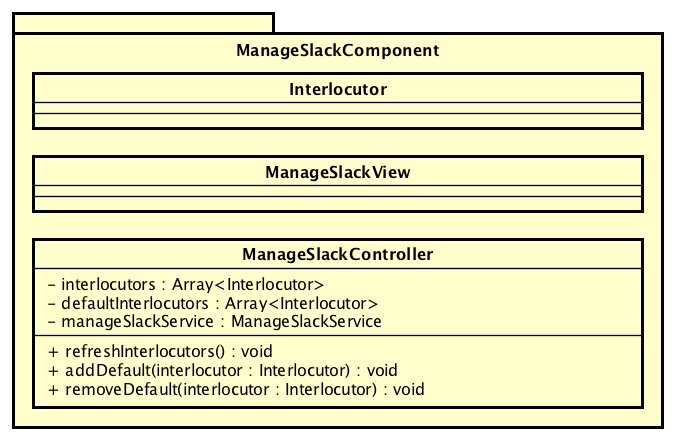
\includegraphics[scale=0.7]{Architettura/Front-End/AdminPage/AdminComponents/ManageSlackComponent.png}
		\caption{Schema del componente \texttt{Front-End :: AdminPage :: AdminComponents :: ManageSlackComponent}}
	\end{figure}
			\subparagraph{Descrizione}: Componente che contiene al suo interno la sua view, il suo controller, ed i models di cui necessita
			\subparagraph{Padre}: AdminComponents
			      \paragraph{\texttt{Front-End :: AdminPage :: AdminComponents :: ManageSlackComponent :: ManageSlackController}}
			      	\subparagraph{Descrizione}: Componente per la gestione dei canali Slack
			      	\subparagraph{Utilizzo}: Componente per la gestione dei canali Slack
			      	\subparagraph{Attributi}:
					\begin{itemize}
						\item \texttt{defaultInterlocutors: Array<Interlocutor>}: Attributo che indica gli interlocutori presenti nel sistema che fanno parte della lista di default del canale \#azienda.
						\item \texttt{interlocutor: Array<Interlocutor>}: Attributo che indica gli interlocutori presenti nel sistema.
						\item \texttt{manageSlackService: ManageSlackService}: Attributo che rappresenta una istanza del service ManageSlackService e ne mette a disposizione i metodi.
					\end{itemize}
	      			\subparagraph{Metodi}:
					\begin{itemize}
						\item \texttt{refreshInterlocutors}
						\subparagraph{Descrizione}:Funzione che permette di aggiornare la lista degli interlocutori nel sistema dal team Slack

						\item \texttt{addDafault}
						\subparagraph{Descrizione}Funzione che permette di aggiungere un interlocutore alla lista di default \#azienda
						\subparagraph{Argomenti}:
						\begin{itemize}
							\item \texttt{interlocutor : Interlocutor}: Parametro che indica l'interlocutore da associare alla lista di default.
						\end{itemize}

						\item \texttt{removeDafault}
						\subparagraph{Descrizione}:Funzione che permette di rimuovere un interlocutore alla lista di default \#azienda
						\subparagraph{Argomenti}:
						\begin{itemize}
							\item \texttt{interlocutor : Interlocutor}: Parametro che indica l'interlocutore da disassociare alla lista di default.
						\end{itemize}
					\end{itemize}
		      	\paragraph{\texttt{Front-End :: AdminPage :: AdminComponents :: ManageSlackComponent :: ManageSlackView}}
					\subparagraph{Descrizione}: View del componente per la gestione dei canali Slack
					\subparagraph{Utilizzo}: View di ManageSlack

	\newpage
	\subsubsection{\texttt{Front-End :: AdminPage :: AdminComponents :: UpdatePasswordComponent}}
	\begin{figure}[!h]
		\centering
		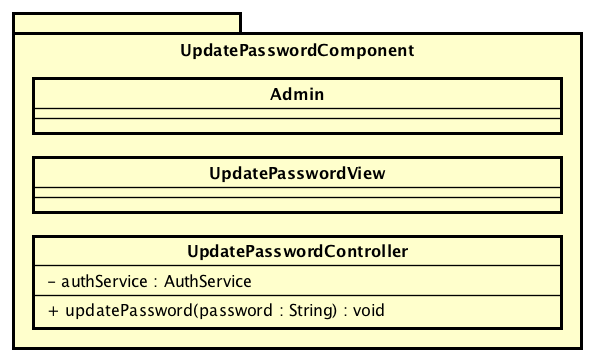
\includegraphics[scale=0.7]{Architettura/Front-End/AdminPage/AdminComponents/UpdatePasswordComponent.png}
		\caption{Schema del componente \texttt{Front-End :: AdminPage :: AdminComponents :: UpdatePasswordComponent}}
	\end{figure}

			\subparagraph{Descrizione}: Componente che contiene al suo interno la sua view, il suo controller, ed i models di cui necessita
			\subparagraph{Padre}: AdminComponents
				\paragraph{\texttt{Front-End :: AdminPage :: AdminComponents :: UpdatePasswordComponent :: UpdatePasswordController}}
					\subparagraph{Descrizione}: Controller che gestisce la view di UpdatePasswordView permettendo ad un amministratore di effettuare l'aggiornamento della propria password previa email ricevuta nella propria casella di posta
					\subparagraph{Utilizzo}: Metodo utilizzato per gestire il cambio della propria password da parte di un Admin
					\subparagraph{Attributi}:
					\begin{itemize}
						\item \texttt{authService: AuthService}: Attributo che rappresenta una istanza del service AuthService e ne mette a disposizione i metodi.
					\end{itemize}
					\subparagraph{Metodi}:
					\begin{itemize}
						\item \texttt{updatePassword(password : string) : void}:
						\subparagraph{Descrizione}:Funzione che permette all'amministratore di aggiornare la propria password
						\subparagraph{Argomenti}:
					  	\begin{itemize}
					  		\item \texttt{password : string}: Parametro che indica la nuova password inserita dall'amministratore.
					  	\end{itemize}
					\end{itemize}\vspace{0.5em}
				\paragraph{\texttt{Front-End :: AdminPage :: AdminComponents :: UpdatePasswordComponent :: UpdatePasswordView}}

		      		\subparagraph{Descrizione}: View di UpdatePassword, permette ad un amministratore di effettuare l'aggiornamento della propria password previa email ricevuta nella propria casella di posta
			      	\subparagraph{Utilizzo}: View di UpdatePasword


	\newpage
	\subsubsection{\texttt{Front-End :: AdminPage :: AdminComponents :: ListViewComponent}}
	\begin{figure}[!h]
		\centering
		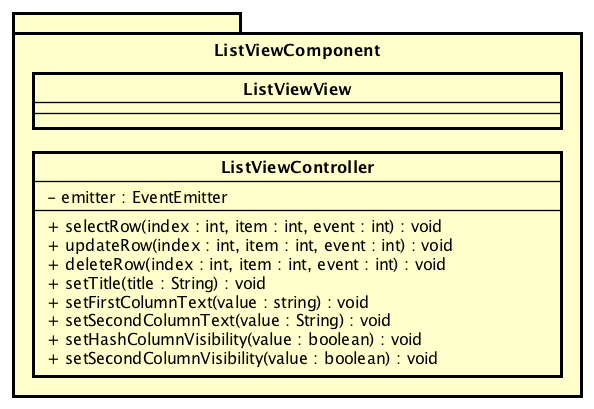
\includegraphics[scale=0.7]{Architettura/Front-End/AdminPage/AdminComponents/ListViewComponent.png}
		\caption{Schema del componente \texttt{Front-End :: AdminPage :: AdminComponents :: ListViewComponent}}
	\end{figure}

			\subparagraph{Descrizione}: Componente che contiene al suo interno la sua view, il suo controller, ed i models di cui necessita
			\subparagraph{Padre}: AdminComponents
			      \paragraph{\texttt{Front-End :: AdminPage :: AdminComponents :: ListViewComponent :: ListViewController}}
			      	\subparagraph{Descrizione}: Controller che gestisce la view di ListViewComponent permettendo di gestire la lista dell'area amministrativa in tutti i contesti in qui viene chiamata in causa
			      	\subparagraph{Utilizzo}: Verrà utilizzato dall'amministratore per gestire le liste presenti nell'area amministrativa
			      	\subparagraph{Attributi}:
			      	      \begin{itemize}
			      	      	\item \texttt{emitter: EventEmitter<any>}: Attributo che rappresenta un'istanza di EventEmitter e ne mette a disposizione i relativi metodi.
			      	      \end{itemize}
			      	\subparagraph{Metodi}:
			      	      \begin{itemize}
			      	      	\item \texttt{setSelectedRow}:
							\subparagraph{Descrizione}:Funzione che permette di ottenere la riga selezionata dalla lista ed emanare un evento 'select' al componente padre
			      	      	\subparagraph{Argomenti}:
			      	      	      \begin{itemize}
			      	      	      	\item \texttt{index : int}: Parametro che indica il numero della riga selezionata.
			      	      	      	\item \texttt{item : any}: Parametro che indica l'oggetto relativo alla riga selezionata.
			      	      	      	\item \texttt{event : string}: Parametro utilizzato per bloccare la propagazione dell'evento propagato dal click.
			      	      	      \end{itemize}
			      	      	\item \texttt{updateRow}:
							\subparagraph{Descrizione}:Funzione che permette di ottenere la riga selezionata dalla lista in base al click del button update ed emanare un evento 'udpate' al componente padre
			      	      	\subparagraph{Argomenti}:
			      	      	      \begin{itemize}
			      	      	      	\item \texttt{index : int}: Parametro che indica il numero della riga selezionata.
			      	      	      	\item \texttt{item : any}: Parametro che indica l'oggetto relativo alla riga selezionata.
			      	      	      	\item \texttt{event : string}: Parametro utilizzato per bloccare la propagazione dell'evento propagato dal click.
			      	      	      \end{itemize}

			      	      	\item \texttt{deleteRow}:
							\subparagraph{Descrizione}:Funzione che permette di ottenere la riga selezionata dalla lista in base al click del button delete ed emanare un evento 'delete' al componente padre
			      	      	\subparagraph{Argomenti}:
			      	      	      \begin{itemize}
			      	      	      	\item \texttt{index : int}: Parametro che indica il numero della riga selezionata.
			      	      	      	\item \texttt{item : any}: Parametro che indica l'oggetto relativo alla riga selezionata.
			      	      	      	\item \texttt{event : string}: Parametro utilizzato per bloccare la propagazione dell'evento propagato dal click.
			      	      	      \end{itemize}
			      	      	\item \texttt{setTitle}:
							\subparagraph{Descrizione}:Funzione che permette di impostare il titolo alla lista
							\subparagraph{Argomenti}:
			      	      	      \begin{itemize}
			      	      	      	\item \texttt{title:string : int}: Parametro che indica il numero della riga selezionata.
			      	      	      \end{itemize}
			      	      	\item \texttt{setFirstColumnText}:
							\subparagraph{Descrizione}:Funzione che permette di impostare il titolo alla prima colonna della lista
							\subparagraph{Argomenti}:
			      	      	      \begin{itemize}
			      	      	      	\item \texttt{title : string}: Parametro che indica il numero della riga selezionata.
			      	      	      \end{itemize}
			      	      	\item \texttt{setSecondColumnText}:
							\subparagraph{Descrizione}:Funzione che permette di impostare il titolo alla seconda colonna della lista

			      	      	\item \texttt{setHashColumnText}:
							\subparagraph{Descrizione}:Funzione che permette di impostare il titolo alla colonna estrema di sinistra della lista

			      	      	\item \texttt{setHashColumnVisibility}:
							\subparagraph{Descrizione}:Funzione che permette di impostare la visibilità della colonna estrema di sinistra della lista
			      	      	\item \texttt{setSecondColumnVisibility}:
							\subparagraph{Descrizione}:Funzione che permette di impostare la visibilità della seconda colonna della lista
			      \end{itemize}
			      \paragraph{\texttt{Front-End :: AdminPage :: AdminComponents :: ListViewComponent :: ListViewView}}
			      	\subparagraph{Descrizione}: View di ListViewComponent, permette di gestire la lista dell'area amministrativa
			      	\subparagraph{Utilizzo}: View di ListViewComponent
\newpage
	\subsubsection{\texttt{Front-End :: AdminPage :: AdminComponents :: ModalViewComponent}}
	\begin{figure}[!h]
		\centering
		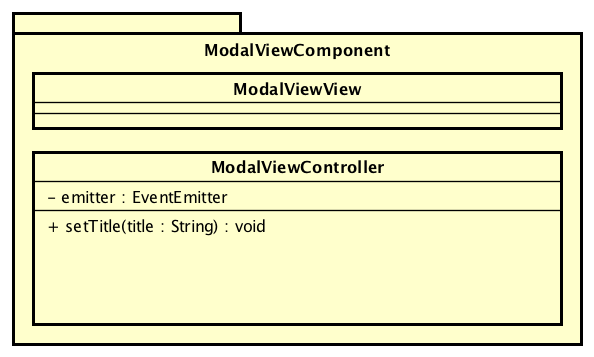
\includegraphics[scale=0.7]{Architettura/Front-End/AdminPage/AdminComponents/ModalViewComponent.png}
		\caption{Schema del componente \texttt{Front-End :: AdminPage :: AdminComponents :: ModalViewComponent}}
	\end{figure}

			\subparagraph{Descrizione}: Componente che contiene al suo interno la sua view, il suo controller, ed i models di cui necessita
			\subparagraph{Padre}: AdminComponents
				\paragraph{\texttt{Front-End :: AdminPage :: AdminComponents :: ModalViewComponent :: ModalViewController}}

					\subparagraph{Descrizione}: Controller che gestisce la view di ModalViewComponent permettendo di gestire il model dell'area amministrativa in tutti i contesti in qui viene chiamato in causa
					\subparagraph{Utilizzo}: Verrà utilizzato dall'amministratore per gestire i form atti ad inserire nuove istanze di un oggetto presenti nell'area amministrativa
					\subparagraph{Attributi}:
					      \begin{itemize}
			      	      	\item \texttt{emitter: EventEmitter<any>}: Attributo che rappresenta un'istanza di EventEmitter e ne mette a disposizione i relativi metodi.
			      	      \end{itemize}
					\subparagraph{Metodi}:
					      \begin{itemize}
			      	      	\item \texttt{setTitle(title : string)}:

							\subparagraph{Descrizione}: Funzione che permette di impostare il titolo al model
							\subparagraph{Argomenti}
							\begin{itemize}
								\item	\texttt{title:string}
							\end{itemize}
			      	      	\item \texttt{getFormValue}:
							\subparagraph{Descrizione}:Funzione che permette di ottenere i valori del form al click del button 'Conferma'
			      	      \end{itemize}\vspace{0.5em}

				\subparagraph{\texttt{Front-End :: AdminPage :: AdminComponents :: ModalViewComponent :: ModalViewController}}
					\subparagraph{Descrizione}: View di ModalViewComponent, permette di gestire il model dell'area amministrativa
					\subparagraph{Utilizzo}: View di ModalViewComponent


	\newpage
	\subsubsection{\texttt{Front-End :: AdminPage :: AdminServices}}

			\subparagraph{Descrizione}: Package che fornisce tutti i servizi utilizzabili da un amministratore ed un super amministratore nella view del Front-End
			\subparagraph{Padre}: AdminPage

				\paragraph{\texttt{Front-End :: AdminPage :: AdminServices :: ManageAdministratorsService}}
				\acapo
				\begin{figure}[!h]
					\centering
					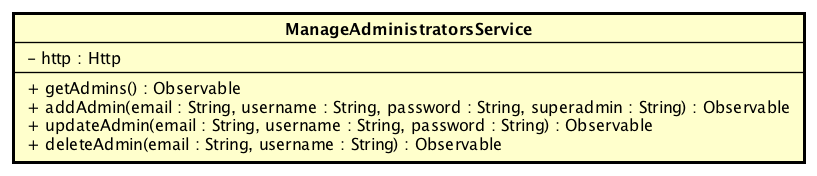
\includegraphics[scale=0.7]{Architettura/Front-End/AdminPage/AdminServices/ManageAdministratorsService.png}
					\caption{Schema del service \texttt{Front-End :: AdminPage :: AdminServices :: ManageAdministratorsService}}
				\end{figure}

					\subparagraph{Descrizione}: Servizi per i componenti del client dell'Admin e del SuperAdmin.
					\subparagraph{Utilizzo}: Gestione servizi Admin e SuperAdmin.
					\subparagraph{Attributi}:
					\begin{itemize}
						\item \texttt{http: Http}: Attributo che rappresenta un'istanza di Http e ne mette a disposizione i relativi metodi.
						\item \texttt{BASE\_PATH: string}: Indirizzo base per le API.
						\item \texttt{PATH:string}: Indirizzo per le API Specifico per il servizio.
					\end{itemize}
					\subparagraph{Metodi}:
					\begin{itemize}
						\item \texttt{getAdmins() : Observable}:
						\subparagraph{Descrizione}:Permette di ottenere tutti gli amministratori presenti nel sistema tramite una chiamata alle API. Ritorna un oggetto di tipo Observable per gestire il risultato della chiamata all'API.

						\item \texttt{addAdmin() : Observable}:

						\subparagraph{Descrizione}:Permette di aggiunge un amministratore con i relativi dati tramite una chiamata alle API. Ritorna un oggetto di tipo Observable per gestire il risultato della chiamata all'API.
						\subparagraph{Parametri}\begin{itemize}
							\item \texttt{email : string}
							\item \texttt{username : string}
							\item \texttt{password : string}
							\item \texttt{superAdmin : boolean}
						\end{itemize}
						\item \texttt{updateAdmin: Observable}:
						\subparagraph{Descrizione}:Permette di aggiornare un amministratore con i relativi dati tramite una chiamata alle API. Ritorna un oggetto di tipo Observable per gestire il risultato della chiamata all'API.
						\subparagraph{Parametri}\begin{itemize}
							\item \texttt{email : string}
							\item \texttt{username : string}
							\item \texttt{password : string}
						\end{itemize}

						\item \texttt{deleteAdmin : Observable}:
						\subparagraph{Descrizione}:Permette di eliminare un amministratore tramite i relativi dati tramite una chiamata alle API. Ritorna un oggetto di tipo Observable per gestire il risultato della chiamata all'API.
						\subparagraph{Parametri}\begin{itemize}
							\item \texttt{email : string}
							\item \texttt{username : string}
						\end{itemize}
					\end{itemize}

\newpage
		      	\paragraph{\texttt{Front-End :: AdminPage :: AdminServices :: ManageFirmsService}}
		      	\acapo
				\begin{figure}[!h]
					\centering
					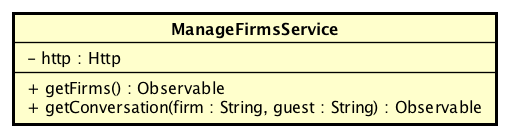
\includegraphics[scale=0.7]{Architettura/Front-End/AdminPage/AdminServices/ManageFirmsService.png}
					\caption{Schema del service \texttt{Front-End :: AdminPage :: AdminServices :: ManageFirmsService}}
				\end{figure}
			      	\subparagraph{Descrizione}: Gestione servizi per i componenti client che si occupano delle aziende.
			      	\subparagraph{Utilizzo}: Utilizzato per gestire le aziende.
			      	\subparagraph{Attributi}:
      	      		\begin{itemize}
						\item \texttt{http: Http}: Attributo che rappresenta un'istanza di Http e ne mette a disposizione i relativi metodi.
						\item \texttt{BASE\_PATH: string}: Indirizzo base per le API.
						\item \texttt{PATH:string}: Indirizzo per le API Specifico per il servizio.
	      	      	\end{itemize}
			      	\subparagraph{Metodi}:
	      	      	\begin{itemize}
						\item \texttt{getFirms : Observable}
						\subparagraph{Descrizione}:Permette di ottenere tutte le aziende e relativi ospiti presenti nel sistema tramite una chiamata alle API. Ritorna un oggetto di tipo Observable per gestire il risultato della chiamata all'API.
						\item \texttt{getConversation : Observable}
						\subparagraph{Descrizione}:Permette di ottenere una conversazione di un ospite tramite una chiamata alle API. Ritorna un oggetto di tipo Observable per gestire il risultato della chiamata all'API.
						\subparagraph{Parametri}\begin{itemize}
							\item \texttt{firm : string}
							\item \texttt{guest : string}
						\end{itemize}
	      	      	\end{itemize}

					\newpage
				\paragraph{\texttt{Front-End :: AdminPage :: AdminServices :: ManageQuestionsService}}
				\acapo
				\begin{figure}[!h]
					\centering
					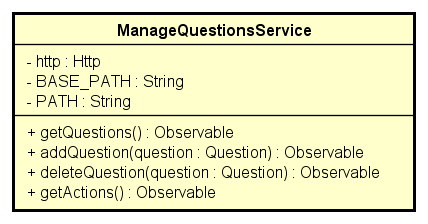
\includegraphics[scale=0.7]{Architettura/Front-End/AdminPage/AdminServices/ManageQuestionsService.png}
					\caption{Schema del service \texttt{Front-End :: AdminPage :: AdminServices :: ManageQuestionsService}}
				\end{figure}

					\subparagraph{Descrizione}: Classe che fornisce funzionalità per la gestione delle domande e delle interazioni collegate ad esse
					\subparagraph{Utilizzo}: Utilizzata per operazioni di gestione delle domande e relative interazioni
					\subparagraph{Attributi}:
			      	\begin{itemize}
						\item \texttt{http: Http}: Attributo che rappresenta un'istanza di Http e ne mette a disposizione i relativi metodi.
						\item \texttt{BASE\_PATH: string}: Indirizzo base per le API.
						\item \texttt{PATH:string}: Indirizzo per le API Specifico per il servizio.
			      	\end{itemize}
					\subparagraph{Metodi}:
	      	      	\begin{itemize}
						\item \texttt{getQuestions : Observable}:
						\subparagraph{Descrizione}:Permette di ottenere tutte le domande e relative risposte presenti nel sistema tramite una chiamata alle API. Ritorna un oggetto di tipo Observable per gestire il risultato della chiamata all'API.

						\item \texttt{getActions : Observable}:
						\subparagraph{Descrizione}:Permette di ottenere tutte le action presenti nel sistema tramite una chiamata alle API. Ritorna un oggetto di tipo Observable per gestire il risultato della chiamata all'API.


						\item \texttt{addQuestion : Observable}
						\subparagraph{Descrizione}:Permette di aggiungere una domanda con relative risposte al sistema tramite una chiamata alle API. Ritorna un oggetto di tipo Observable per gestire il risultato della chiamata all'API.
						\subparagraph{Parametri}\begin{itemize}
							\item \texttt{question : Question}
						\end{itemize}

						\item \texttt{addQuestion : Observable}
						\subparagraph{Descrizione}:Permette di rimuovere una domanda con relative risposte dal sistema tramite una chiamata alle API. Ritorna un oggetto di tipo Observable per gestire il risultato della chiamata all'API.
						\subparagraph{Parametri}\begin{itemize}
							\item \texttt{question : Question}
						\end{itemize}

						
	      	      	\end{itemize}
\newpage

     	 		\paragraph{\texttt{Front-End :: AdminPage :: AdminServices :: ManageSlackService}}
     	 		\acapo
				\begin{figure}[!h]
					\centering
					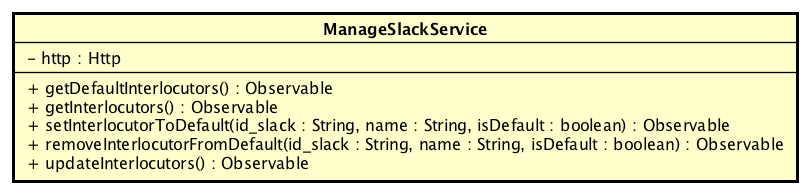
\includegraphics[scale=0.7]{Architettura/Front-End/AdminPage/AdminServices/ManageSlackService.png}
					\caption{Schema del service \texttt{Front-End :: AdminPage :: AdminServices :: ManageSlackService}}
				\end{figure}

				\subparagraph{Descrizione}: Gestione servizi lato client dei componenti che si interfacciano ai servizi di Slack.
				\subparagraph{Utilizzo}: Utilizzato per gestire i servizi di interfaccia ai servizi di Slack.
				\subparagraph{Attributi}:
				\begin{itemize}
					\item \texttt{http: Http}: Attributo che rappresenta un'istanza di Http e ne mette a disposizione i relativi metodi.
					\item \texttt{BASE\_PATH: string}: Indirizzo base per le API.
					\item \texttt{PATH:string}: Indirizzo per le API Specifico per il servizio.
				\end{itemize}
				\subparagraph{Metodi}:
				\begin{itemize}
					\item \texttt{getDefaultInterlocutors : Observable}
					\subparagraph{Descrizione}:Permette di ottenere tutti gli interlocutori presenti nel sistema e facenti parte della lista di default \#azienda tramite una chiamata alle API. Ritorna un oggetto di tipo Observable per gestire il risultato della chiamata all'API.

					\item \texttt{getInterlocutors : Observable}
					\subparagraph{Descrizione}:Permette di ottenere tutti gli interlocutori presenti nel sistema tramite una chiamata alle API. Ritorna un oggetto di tipo Observable per gestire il risultato della chiamata all'API.

					\item \texttt{setInterlocutorToDefault : Observable}
					\subparagraph{Descrizione}:Permette di impostare un interlocutore, già presente nel sistema, come facente parte della lista di default \#azienda tramite una chiamata alle API. Ritorna un oggetto di tipo Observable per gestire il risultato della chiamata all'API.
						\subparagraph{Parametri}\begin{itemize}
							\item \texttt{id\_slack : string}
							\item \texttt{name : string}
						\end{itemize}
					\item \texttt{removeInterlocutorFromDefault : Observable}
					\subparagraph{Descrizione}:Permette di disassociare un interlocutore, già presente nel sistema, dalla lista di default \#azienda tramite una chiamata alle API. Ritorna un oggetto di tipo Observable per gestire il risultato della chiamata all'API.
						\subparagraph{Parametri}\begin{itemize}
							\item \texttt{id\_slack : string}
							\item \texttt{name : string}
						\end{itemize}
					\item \texttt{updateInterlocutors : Observable}
					\subparagraph{Descrizione}:Permette di ottenere gli interlocutori aggiornati presententi nel team Slack associato tramite una chiamata alle API. Ritorna un oggetto di tipo Observable per gestire il risultato della chiamata all'API.
				\end{itemize}

				\newpage
		      	\paragraph{\texttt{Front-End :: AdminPage :: AdminServices :: AuthService}}
		      	\acapo
				\begin{figure}[!h]
					\centering
					\includegraphics[scale=0.7]{Architettura/Front-End/AdminPage/AdminServices/AuthService.png}
					\caption{Schema del service \texttt{Front-End :: AdminPage :: AdminServices :: AuthService}}
				\end{figure}

				\subparagraph{Descrizione}: Classe che fornisce servizi per effettuare operazioni di autenticazione nel client dell'Admin e del SuperAdmin
				\subparagraph{Utilizzo}: Utilizzata quando un amministratore o un super amministratore effettua operazioni di autenticazione nell'interfaccia
				\subparagraph{Attributi}:
				\begin{itemize}
					\item \texttt{http: Http}: Attributo che rappresenta un'istanza di Http e ne mette a disposizione i relativi metodi.
					\item \texttt{BASE\_PATH: string}: Indirizzo base per le API.
					\item \texttt{PATH:string}: Indirizzo per le API Specifico per il servizio.
				\end{itemize}
				\subparagraph{Metodi}:
				\begin{itemize}
					\item \texttt{login : Observable}
					\subparagraph{Descrizione}:Permette ad un amministratore di effettuare il login tramite una chiamata alle API. Ritorna un oggetto di tipo Observable per gestire il risultato della chiamata all'API.
					\subparagraph{Parametri}\begin{itemize}
						\item \texttt{username : string}
						\item \texttt{password : string}
					\end{itemize}

					\item \texttt{update : Observable}
					\subparagraph{Descrizione}: Permette ad un amministratore di aggiornare alcuni dati del proprio profilo tramite una chiamata alle API. Ritorna un oggetto di tipo Observable per gestire il risultato della chiamata all'API.
					\subparagraph{Parametri}\begin{itemize}
						\item \texttt{username : string}
						\item \texttt{password : string}
					\end{itemize}
					\item \texttt{logout : Observable}
					\subparagraph{Descrizione}:Permette ad un amministratore di effettuare il logout tramite una chiamata alle API. Ritorna un oggetto di tipo Observable per gestire il risultato della chiamata all'API.

					\item \texttt{checkToken : Observable}:
					\subparagraph{Descrizione}:Permette ad un amministratore di verificare se il token a lui associato in fase di login è ancora valido tramite una chiamata alle API. Ritorna un oggetto di tipo Observable per gestire il risultato della chiamata all'API.
				\end{itemize}

	\newpage
	\subsubsection{\texttt{Front-End :: GuestPage}}
	\begin{figure}[!h]
		\centering
		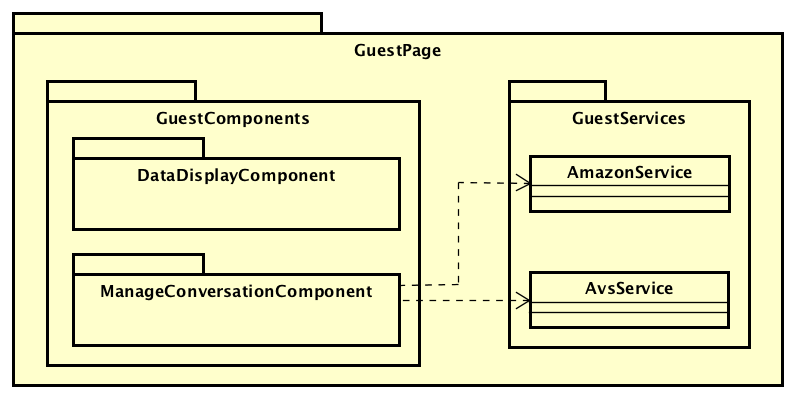
\includegraphics[scale=0.7]{Architettura/Front-End/GuestPage/GuestPage.png}
		\caption{Schema del componente \texttt{Front-End :: GuestPage}}
	\end{figure}

			\subparagraph{Descrizione}: Package dedicato alla parte d'interfaccia client disponibile all'ospite
			\subparagraph{Padre}: Front-End
			\subparagraph{Package contenuti}:
			\begin{itemize}
				\item Front-End :: GuestPage :: GuestComponents: Package dedicato alla parte view e controller dell'interfaccia ospite
				\item Front-End :: GuestPage :: GuestServices: Package dedicato ai servizi resi disponibili a GuestComponents
			\end{itemize}


	\newpage
	\subsubsection{\texttt{Front-End :: GuestPage :: GuestComponents}}

			\subparagraph{Descrizione}: Package dedicato alla parte view e controller dell'interfaccia ospite
			\subparagraph{Padre}: GuestPage
			\subparagraph{Package contenuti}:
			\begin{itemize}
				\item Front-End :: GuestPage :: GuestComponents :: ManageConversationComponent: Componente che contiene al suo interno la sua view, il suo controller, ed i models di cui necessita
				\item Front-End :: GuestPage :: GuestComponents :: DataDisplayComponent: Componente che contiene al suo interno la sua view, il suo controller, ed i models di cui necessita
			\end{itemize}

	\newpage
	\subsubsection{\texttt{Front-End :: GuestPage :: GuestComponents :: ManageConversationComponent}}
	\begin{figure}[!h]
		\centering
		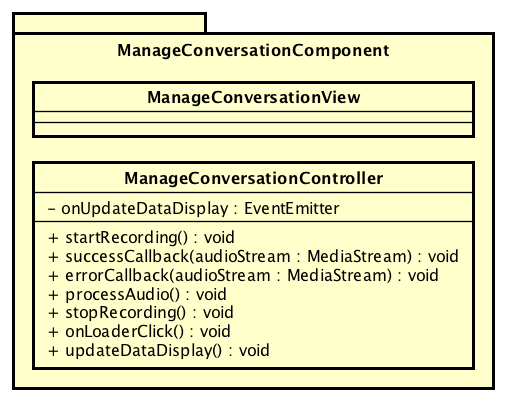
\includegraphics[scale=0.7]{Architettura/Front-End/GuestPage/GuestComponents/ManageConversationComponent.png}
		\caption{Schema del componente \texttt{Front-End :: GuestPage :: GuestComponents :: ManageConversationComponent}}
	\end{figure}

			\subparagraph{Descrizione}: Componente che contiene al suo interno la sua view, il suo controller, ed i models di cui necessita
			\subparagraph{Padre}: GuestComponents

			\paragraph{\texttt{Front-End :: GuestPage :: GuestComponents :: ManageConversationComponent :: ManageConversationController}}

				\subparagraph{Descrizione}: Classe che si occupa di gestire la conversazione tra ospite e sistema
				\subparagraph{Utilizzo}: Sarà utilizzata per permettere la conversazione tra ospite e Assistente Virtuale
				\subparagraph{Attributi}:
				\begin{itemize}
					\item \texttt{onUpdateDataDisplay : EventEmitter<any>}: Attributo che rappresenta un'istanza di EventEmitter e ne mette a disposizione i relativi metodi.
				\end{itemize}
				\subparagraph{Metodi}:
				\begin{itemize}
					\item \texttt{startRecording : void}
					\subparagraph{Descrizione}:Funzione utilizzata per cominciare la registrazione dell'audio inizializzando lo stream audio

					\item \texttt{successCallback : void}
					\subparagraph{Descrizione}: Funzione utilizzata come callback di startRecording(), invocata quando lo stream audio è stato inizializzato ed è pronto ad essere utilizzato per la registrazione
					\subparagraph{Parametri}\begin{itemize}
						\item \texttt{audioStream : MediaStream}
					\end{itemize}

					\item \texttt{errorCallback : void}
					\subparagraph{Descrizione}: Funzione utilizzata come callback di startRecording(), invocata quando non è stato possibile inizializzare lo stream audio (ad esempio se il microfono non è presente nel device)
					\subparagraph{Parametri}\begin{itemize}
						\item \texttt{audioStream : MediaStream}
					\end{itemize}

					\item \texttt{processAudio : void}
					\subparagraph{Descrizione}: Funzione invocata al termine della registrazione ed utilizzata per elaborare lo stream audio in base al formato impostato via codice

					\item \texttt{stopRecording : void}
					\subparagraph{Descrizione}: Funzione utilizzata per interrompere la registrazione dello stream audio

					\item \texttt{onLoaderClick : void}
					\subparagraph{Descrizione}: Funzione utilizzata iniziare o interrompere la conversazione manualmente. A sua volte invocherà quindi startRecording() o stopRecording()

					\item \texttt{updateDataDisplay : void}
					\subparagraph{Descrizione}: Funzione utilizzata per emettere un evento, utilizzando onUpdateDataDisplay, al componente padre, passando informazioni come del testo da mostrare a video o un elenco di aziende da suggerire all'ospite
				\end{itemize}

			\paragraph{\texttt{Front-End :: GuestPage :: GuestComponents :: ManageConversationComponent :: ManageConversationView}}

				\subparagraph{Descrizione}: Classe utilizzata per visualizzare la conversazione tra ospite e AV
				\subparagraph{Utilizzo}: View di ManageConversationComponent



	\newpage
	\subsubsection{\texttt{Front-End :: GuestPage :: GuestComponents :: DataDisplayComponent}}
	\begin{figure}[!h]
		\centering
		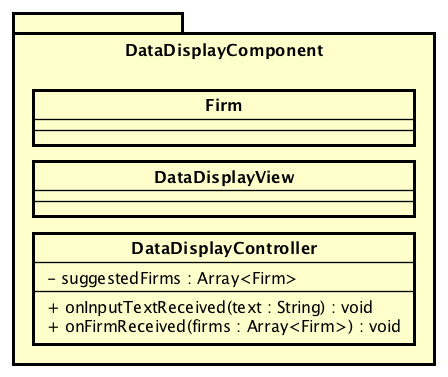
\includegraphics[scale=0.7]{Architettura/Front-End/GuestPage/GuestComponents/DataDisplayComponent.png}
		\caption{Schema del componente \texttt{Front-End :: GuestPage :: GuestComponents :: DataDisplayComponent}}
	\end{figure}

			\subparagraph{Descrizione}: Componente che contiene al suo interno la sua view, il suo controller, ed i models di cui necessita
			\subparagraph{Padre}: GuestComponents

			\paragraph{\texttt{Front-End :: GuestPage :: GuestComponents :: DataDisplayComponent :: DataDisplayController}}
				\subparagraph{Descrizione}: Classe contenente tutti i metodi necessari a mostrare a schermo informazioni utili all'ospite
				\subparagraph{Utilizzo}: Verrà utilizzata per fornire informazioni all'utente o ospite
				\subparagraph{Attributi}:
				\begin{itemize}
					\item \texttt{sugestedFirms: Array<Firm>}: Attributo di appoggio che indica un array di aziende da mostrare a video all'ospite
				\end{itemize}
				\subparagraph{Metodi}:
				\begin{itemize}
					\item \texttt{onInputTextReceived}
					\subparagraph{Descrizione}:Funzione utilizzata per ottenere e mostrare a video il testo che Alexa ha compreso
					\subparagraph{Parametri}\begin{itemize}
						\item \texttt{text : string}
					\end{itemize}

					\item \texttt{onFirmsReceived}
					\subparagraph{Descrizione}:Funzione che riceve e mostra a video le aziende da suggerire all'utente
					\subparagraph{Parametri}\begin{itemize}
						\item \texttt{firms : Array<Firm>}
					\end{itemize}

				\end{itemize}\vspace{0.5em}
			\paragraph{\texttt{Front-End :: GuestPage :: GuestComponents :: DataDisplayComponent :: DataDisplayView}}

				\subparagraph{Descrizione}: Classe contenente tutti i metodi necessari a mostrare a schermo informazioni utili all'utente o ospite
				\subparagraph{Utilizzo}: View di DataDisplayComponent

	\newpage
	\subsubsection{\texttt{Front-End :: GuestPage :: GuestServices}}

			\subparagraph{Descrizione}: Package dedicato ai servizi resi disponibili agli ospiti
			\subparagraph{Padre}: GuestPage

			\paragraph{\texttt{Front-End :: GuestPage :: GuestServices :: AmazonService}}
			\acapo
			\begin{figure}[!h]
				\centering
				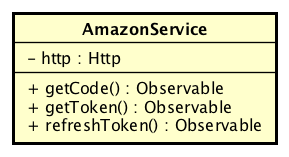
\includegraphics[scale=0.7]{Architettura/Front-End/GuestPage/GuestServices/AmazonService.png}
				\caption{Schema del service \texttt{Front-End :: GuestPage :: GuestServices :: AmazonService}}
			\end{figure}

			\subparagraph{Descrizione}: Contiene i servizi necessari ad effettuare l'autenticazione ad Amazon ed iniziare ad utilizzare Alexa Voice Service
			\subparagraph{Utilizzo}: Servizi per i components dell'interfaccia ospite.
			\subparagraph{Attributi}:
			\begin{itemize}
				\item \texttt{http: Http}: Attributo che rappresenta un'istanza di Http e ne mette a disposizione i relativi metodi.
			\end{itemize}
			\subparagraph{Metodi}:
			\begin{itemize}
				\item \texttt{getCode : Observable}
				\subparagraph{Descrizione}: Primo passaggio per effettuare il Login with Amazon. Restituisce un codice di volta in volta diverso utile a proseguire nel workflow di \gl{LWA}. La stringa ricevuta viene memorizzata nel sessionStorage del browser.

				\item \texttt{getToken : Observable}
				\subparagraph{Descrizione}:Secondo passaggio per effettuare il Login with Amazon. Restituisce un token basato sul code ricevuto nel primo passaggio, utile per tutte le chiamate alle API di Alexa Voice Service, ed un refreshToken utile ad aggiornare la validità del token. Le stringhe ricevute vengono memorizzate nel sessionStorage del browser.

				\item \texttt{refreshToken : Observable}
				\subparagraph{Descrizione}:Funzione utile ad aggiornare il token ricevuto nel secondo passaggio grazie al refreshToken. Il nuovo token viene nuovamente memorizzato nel sessionStorage del browser.
			\end{itemize}


			\newpage
			\paragraph{\texttt{Front-End :: GuestPage :: GuestServices :: AvsService}}
			\acapo
			\begin{figure}[!h]
				\centering
				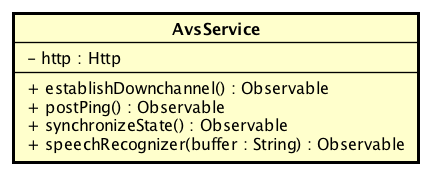
\includegraphics[scale=0.7]{Architettura/Front-End/GuestPage/GuestServices/AvsService.png}
				\caption{Schema del service \texttt{Front-End :: GuestPage :: GuestServices :: AvsService}}
			\end{figure}

				\subparagraph{Descrizione}: Contiene i servizi necessari ad effettuare le chiamate alle API di Alexa Voice Service
				\subparagraph{Utilizzo}: Servizi per i components dell'interfaccia ospite.
				\subparagraph{Attributi}:
				\begin{itemize}
					\item \texttt{http: Http}: Attributo che rappresenta un'istanza di Http e ne mette a disposizione i relativi metodi.
				\end{itemize}
				\subparagraph{Metodi}:
				\begin{itemize}
					\item \texttt{establishDownchannel : Observable}
					\subparagraph{Descrizione}:Permette di creare un canale Http2 utile a ricevere direttive dal cloud di AVS, tramite una chiamata alle API di Alexa Voice Service

					\item \texttt{postPing : Observable}
					\subparagraph{Descrizione}:Permette di inviare un evento di ping al cloud di AVS, tramite una chiamata alle API di Alexa Voice Service

					\item \texttt{synchronizeState : Observable}
					\subparagraph{Descrizione}:Permette di inviare un evento di Synchronize State al cloud di AVS, tramite una chiamata alle API di Alexa Voice Service

					\item \texttt{speechRecognizer : Observable}
					\subparagraph{Descrizione}:Permette di inviare un evento di Speech Recognizer al cloud di AVS, tramite una chiamata alle API di Alexa Voice Service
					\subparagraph{Argomenti}:
					\begin{itemize}
						\item \texttt{buffer : string}: Parametro che indica il buffer di un file audio sotto forma di stringa binaria
					\end{itemize}
      			\end{itemize}


	\newpage
	\subsection{\texttt{Models}}
		\subparagraph{Descrizione}: Package che contiene tutti i models


	\paragraph{\texttt{Models :: Action}}
	\acapo
	\begin{figure}[!h]
		\centering
		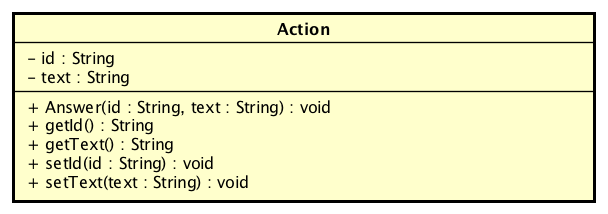
\includegraphics[scale=0.7]{Architettura/Front-End/Models/Action.png}
		\caption{Schema del componente \texttt{Models :: Action}}
	\end{figure}

		\subparagraph{Descrizione}: Rappresenta un'azione predefinita e ne contiene tutte le informazioni necessarie alla presentazione del suo contenuto
		\subparagraph{Utilizzo}: Viene utilizzata per memorizzare i dati di un'azione predefinita
		\subparagraph{Attributi}:
		      \begin{itemize}
		      	\item \texttt{id: string}:
		      	      Attributo che rappresenta l'id di un'azione predefinita.
		      	\item \texttt{text: string}:
		      	      Attributo che rappresenta il testo di un'azione predefinita.
		      \end{itemize}
		\subparagraph{Metodi}:
		      \begin{itemize}
		      	\item \texttt{Action : void}
		      	      \subparagraph{Descrizione}:Costruttore
					\subparagraph{Argomenti}:
						\begin{itemize}
							\item \texttt{id : string}:
								ID dell'Action.
							\item \texttt{text : string}:
								Testo descrittivo dell'Action.
						\end{itemize}

		      	\item \texttt{getId() : string}
		      	      \subparagraph{Descrizione}:Getter dell'ID

		      	\item \texttt{setId() : void}
		      	      \subparagraph{Descrizione}:Setter dell'ID

		      	\item \texttt{setText() : void}
		      	      \subparagraph{Descrizione}:Setter del testo descrittivo

		      	\item \texttt{getText() : string}
		      	      \subparagraph{Descrizione}:Getter del testo descrittivo
		      \end{itemize}



	\newpage
	\paragraph{\texttt{Models :: Admin}}
	\acapo
	\begin{figure}[!h]
		\centering
		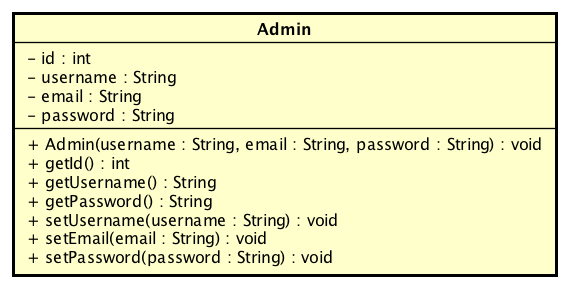
\includegraphics[scale=0.7]{Architettura/Front-End/Models/Admin.png}
		\caption{Schema del componente \texttt{Models :: Admin}}
	\end{figure}

		\subparagraph{Descrizione}: Rappresenta un amministratore e ne contiene tutte le informazioni necessarie alla presentazione del suo contenuto
		\subparagraph{Utilizzo}: Viene utilizzata per memorizzare i dati di un amministratore
		\subparagraph{Attributi}:
		      \begin{itemize}
		      	\item \texttt{email: string}:
		      	      Attributo che rappresenta la email di un amministratore.

		      	\item \texttt{password: string}:
		      	      Attributo che rappresenta la password di un amministratore.

		      	\item \texttt{username: string}:
		      	      Attributo che rappresenta lo username di un amministratore.
		      \end{itemize}
		\subparagraph{Metodi}:
		      \begin{itemize}
		      	\item \texttt{Admin : void}
		      	      \subparagraph{Descrizione}:Costruttore del modello Admin
					\subparagraph{Descrizione}:{Argomenti}:
						\begin{itemize}
							\item \texttt{password : string}:
								Parametro che indica la password dell'amministratore.
							\item \texttt{username : string}:
								Parametro che indica lo username dell'amministratore.
						\end{itemize}

		      	\item \texttt{getEmail : string}:
		      	      \subparagraph{Descrizione}:Funzione che permette di ottenere l'email dell'amministratore

		      	\item \texttt{getPassword : string}:
		      	      \subparagraph{Descrizione}:Funzione che permette di ottenere la password di un amministratore

		      	\item \texttt{getUsername : string}:
		      	      \subparagraph{Descrizione}:Funzione che permette di ottenere lo username di un amministratore

		      	\item \texttt{setEmail}:
		      	     	\subparagraph{Descrizione}: Funzione che permette di modificare la email di un amministratore
					\subparagraph{Argomenti}:
						\begin{itemize}
							\item \texttt{email : string}:
								Parametro che indica la nuova email di un amministratore.
						\end{itemize}

		      	\item \texttt{setPassword}:
		      	     	\subparagraph{Descrizione}: Funzione che permette di modificare la password di un amministratore
					\subparagraph{Argomenti}:
						\begin{itemize}
							\item \texttt{password : string}:
								Parametro che indica la nuova password di un amministratore.
						\end{itemize}

		      	\item \texttt{setUsername(username) : void}:
		      	      \subparagraph{Descrizione}:Funzione che permette di modificare lo username di un amministratore
					\subparagraph{Argomenti}:
						\begin{itemize}
							\item \texttt{username : string}:
								Parametro che indica il nuovo username dell'amministratore.
						\end{itemize}
			\end{itemize}

		\subparagraph{Relazioni con altre classi}:
		      \begin{itemize}
		      	\item \texttt{Front-End :: AdminPage :: AdminComponents :: ManageAdministratorsComponent :: ManageAdministratorsController}: Controller che gestisce la view di ManageAdministrators permettendo ad un SuperAdmin di gestire le informazioni degli altri amministratori;
		      	\item \texttt{Front-End :: AdminPage :: AdminComponents :: ManageProfileComponent :: ManageProfileController}: Controller che gestisce la view di ManageProfileView permettendo ad un amministratore di gestire il proprio profilo nell'area amministrativa.
		      \end{itemize}

	\newpage
	\paragraph{\texttt{Models :: Answer}}
	\acapo
	\begin{figure}[!h]
		\centering
		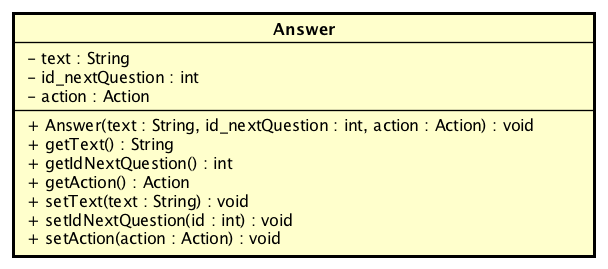
\includegraphics[scale=0.7]{Architettura/Front-End/Models/Answer.png}
		\caption{Schema del componente \texttt{Models :: Answer}}
	\end{figure}

		\subparagraph{Descrizione}: Rappresenta una risposta e ne contiene tutte le informazioni necessarie alla presentazione del suo contenuto
		\subparagraph{Utilizzo}: Viene utilizzata per memorizzare i dati di una risposta
		\subparagraph{Attributi}:
		      \begin{itemize}
		      	\item \texttt{action: Action}:
		      	      Attributo che rappresenta l'azione predefinita da eseguire legata ad una risposta.

		      	\item \texttt{id\_nextQuestion: int}:
		      	      Attributo che rappresenta l'id della prossima domanda legata ad una risposta.

		      	\item \texttt{text: string}:
		      	      Attributo che rappresenta il testo di una risposta.
		      \end{itemize}
		\subparagraph{Metodi}:
		      \begin{itemize}
		      	\item \texttt{Answer}:
		      	      \subparagraph{Descrizione}:Costruttore
					\subparagraph{Descrizione}{Argomenti}:
						\begin{itemize}
							\item \texttt{action : Action}:
								Azione da eseguire.
							\item \texttt{text : string}:
								Testo della risposta.
						\end{itemize}

		      	\item \texttt{getAction : Action}:
		      	      \subparagraph{Descrizione}:Getter dell'azione da eseguire

		      	\item \texttt{getIdNextQuestion : int}:
		      	      \subparagraph{Descrizione}:Getter dell'ID della prossima domanda da porre

		      	\item \texttt{getText : string}:
		      	      \subparagraph{Descrizione}:Getter del testo

		      	\item \texttt{setAction : void}:
		      	      \subparagraph{Descrizione}:Setter dell'Action

		      	\item \texttt{setIdNextQuestion : void}:
		      	      \subparagraph{Descrizione}: Setter dell'ID della prossima domanda da porre
					\subparagraph{Argomenti}:
						\begin{itemize}
							\item \texttt{id : int}:
								ID della prossima domanda.
						\end{itemize}

		      	\item \texttt{setText() : void}:
		      	      \subparagraph{Descrizione}: Setter del testo della risposta
		      \end{itemize}\vspace{0.5em}
		\subparagraph{Relazioni con altre classi}:
		      \begin{itemize}
		      	\item \texttt{Front-End :: AdminPage :: AdminComponents :: ManageQuestionsComponent :: ManageQuestionsController}: Componente per le domande e interazioni.
		      \end{itemize}


\newpage
	\paragraph{\texttt{Models :: Conversation}}
	\acapo
	\begin{figure}[!h]
		\centering
		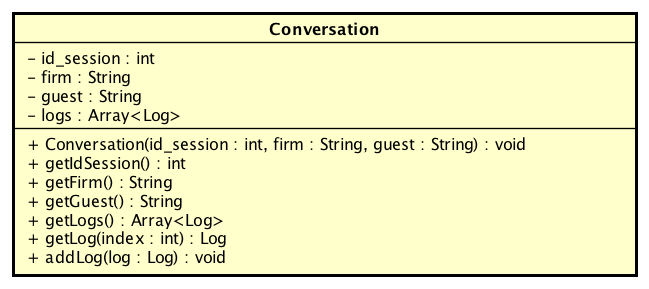
\includegraphics[scale=0.7]{Architettura/Front-End/Models/Conversation.png}
		\caption{Schema del componente \texttt{Models :: Conversation}}
	\end{figure}
		\subparagraph{Descrizione}: Rappresenta una conversazione e ne contiene tutte le informazioni necessarie alla presentazione del suo contenuto
		\subparagraph{Utilizzo}: Viene utilizzata per memorizzare i dati di una conversazione
		\subparagraph{Attributi}:
				\begin{itemize}
					\item \texttt{id\_session: int}: Attributo che rappresenta la session\_id di un conversazione.

					\item \texttt{firm: string}: Attributo che rappresenta il nome dell'azienda

					\item \texttt{guest : string}: Attributo che rappresenta il nominativo di un ospite

					\item \texttt{logs: Array<Log>}: Attributo che rappresenta l'insieme dei log di una conversazione
				\end{itemize}
			\subparagraph{Metodi}:
				\begin{itemize}
					\item \texttt{addLog : void}:
					      \subparagraph{Descrizione}:Funzione che permette di aggiungere un log alla conversazione
						\subparagraph{Argomenti}:
							\begin{itemize}
								\item \texttt{log : Log}:
									Parametro che indica il nuovo log da aggiungere alla conversazione.
							\end{itemize}

					\item \texttt{Conversation : void}:
					      \subparagraph{Descrizione}: Costruttore del model Conversation
						\subparagraph{Argomenti}:
							\begin{itemize}
								\item \texttt{id\_session : int}:
									Parametro che indica l'id\_session della sessione di Alexa.
							\end{itemize}

					\item \texttt{getIdSession : int}:
					      \subparagraph{Descrizione}:Funzione che permette di ottenere l'id\_session di una conversazione

					\item \texttt{getLog : Log}:
					     \subparagraph{Descrizione}: Funzione che permette di ottenere uno specifico log di una conversazione

					\item \texttt{getLogs : Array<Log>}:
						\subparagraph{Descrizione}:Funzione che permette di ottenere l'insieme dei log di una conversazione

					\item \texttt{getFirm : string}:
						\subparagraph{Descrizione}:Funzione che permette di ottenere il nome dell'azienda

					\item \texttt{getGuest : string}:
						\subparagraph{Descrizione}:Funzione che permette di ottenere il nome di un ospite
				\end{itemize}

		\subparagraph{Relazioni con altre classi}:
		      \begin{itemize}
		      	\item \texttt{Front-End :: AdminPage :: AdminComponents :: ManageFirmsComponent :: ManageFirmsController}: Componente per la scelta degli oggetti di tipo Firm.
		      \end{itemize}

\newpage
	\paragraph{\texttt{Models :: Firm}}
	\acapo
	\begin{figure}[!h]
		\centering
		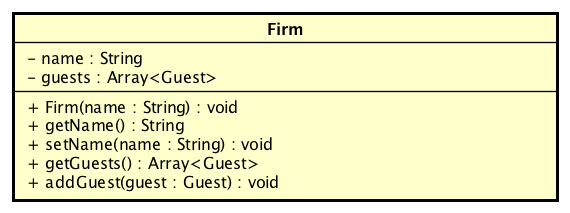
\includegraphics[scale=0.7]{Architettura/Front-End/Models/Firm.png}
		\caption{Schema del componente \texttt{Models :: Firm}}
	\end{figure}


		\subparagraph{Descrizione}: Rappresenta un'azienda e ne contiene tutte le informazioni necessarie alla presentazione del suo contenuto

		\subparagraph{Utilizzo}: Viene utilizzata per memorizzare i dati di un'azienda

		\subparagraph{Attributi}:
		      \begin{itemize}
		      	\item \texttt{guests: Array<Guest>}:
		      	      Attributo che rappresenta gli ospiti registrati di un'azienda.
		      	\item \texttt{id: int}:
		      	      Attributo che rappresenta l'id di un'azienda.
		      	\item \texttt{name: string}:
		      	      Attributo che rappresenta il nome di un'azienda.
		      \end{itemize}

		\subparagraph{Metodi}:
		      \begin{itemize}
		      	\item \texttt{addGuest}:
		      	      \subparagraph{Descrizione}:Funzione che permette di aggiungere un nuovo ospiti ad un'azienda
		      	\subparagraph{Argomenti}:
		      	      \begin{itemize}
		      	      	\item \texttt{guest : Guest}:
		      	      	      Parametro che indica l'ospite da aggiungere all'azienda.
		      	      \end{itemize}

		      	\item \texttt{Firm}:
		      	      \subparagraph{Descrizione}:Costruttore del model azienda
		      	\subparagraph{Argomenti}:
		      	      \begin{itemize}
		      	      	\item \texttt{name : string}:
		      	      	      Parametro che indica il nome di un'azienda.
		      	      \end{itemize}

		      	\item \texttt{getId : int}:
		      	      \subparagraph{Descrizione}Funzione che permette di ottenere l'id di un'azienda

		      	\item \texttt{getName : string}:
		      	      \subparagraph{Descrizione}Funzione che permette di ottenere il nome di un'azienda

		      	\item \texttt{setName}:
		      	      \subparagraph{Descrizione}Funzione che permette di modificare il nome di un'azienda
		      		\subparagraph{Argomenti}:
		      	      \begin{itemize}
		      	      	\item \texttt{name : string}:
		      	      	      Parametro che indica il nuovo nome dell'azienda.
		      	      \end{itemize}
		      \end{itemize}
		\subparagraph{Relazioni con altre classi}:
		      \begin{itemize}
		      	\item \texttt{Front-End :: AdminPage :: AdminComponents :: ManageFirmsComponent :: ManageFirmsController}: Componente per la scelta degli oggetti di tipo Firm.
		      \end{itemize}


	\newpage
	\paragraph{\texttt{Models :: Guest}}
	\acapo
	\begin{figure}[!h]
		\centering
		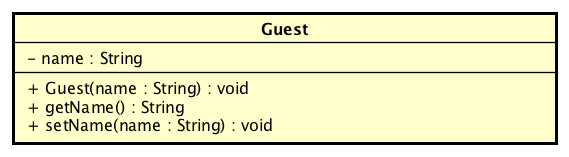
\includegraphics[scale=0.7]{Architettura/Front-End/Models/Guest.png}
		\caption{Schema del componente \texttt{Models :: Guest}}
	\end{figure}

		\subparagraph{Descrizione}: Rappresenta un ospite e ne contiene tutte le informazioni necessarie alla presentazione del suo contenuto
		\subparagraph{Utilizzo}: Viene utilizzata per memorizzare i dati di un ospite
		\subparagraph{Attributi}:
		      \begin{itemize}
		      	\item \texttt{name: string}:
		      	      Attributo che rappresenta il nome di un ospite
		      	      .
		      \end{itemize}
		\subparagraph{Metodi}:
		      \begin{itemize}
		      	\item \texttt{getName : string}:
		      	      \subparagraph{Descrizione}:Funzione che permette di ottenere il nome di un guest

		      	\item \texttt{Guest : void}:
		      	     \subparagraph{Descrizione}: Costruttore del modello Guest

		      	\item \texttt{setName : void}:
		      	      \subparagraph{Descrizione}:Funzione che permette di modificare il nome di un ospite
		      \end{itemize}

		\subparagraph{Relazioni con altre classi}:
		      \begin{itemize}
		      	\item \texttt{Front-End :: AdminPage :: AdminComponents :: ManageFirmsComponent :: ManageFirmsController}: Componente per la scelta degli oggetti di tipo Firm.
		      \end{itemize}

	\newpage
	\paragraph{\texttt{Models :: Interlocutor}}
	\acapo
	\begin{figure}[!h]
		\centering
		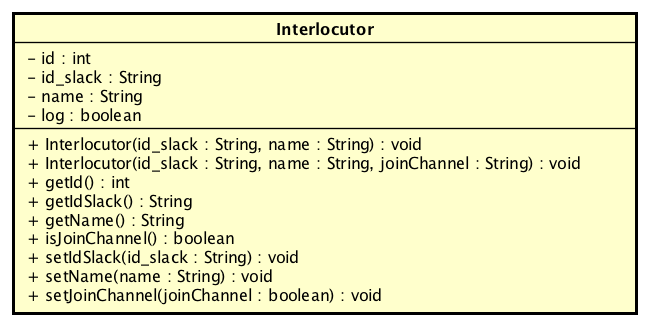
\includegraphics[scale=0.7]{Architettura/Front-End/Models/Interlocutor.png}
		\caption{Schema del componente \texttt{Models :: Interlocutor}}
	\end{figure}

		\subparagraph{Descrizione}: Rappresenta un interlocutore e ne contiene tutte le informazioni necessarie alla presentazione del suo contenuto
		\subparagraph{Utilizzo}: Viene utilizzata per memorizzare i dati di un interlocutore
		\subparagraph{Attributi}:
			\begin{itemize}
				\item \texttt{id\_slack: string}: Attributo che rappresenta l'id di Slack di un interlocutore

				\item \texttt{default: boolean}: Attributo che indica se un interlocutore è associato o meno alla lista di default \#azienda.

				\item \texttt{name: string}: Attributo che rappresenta il nome di un interlocutore
			\end{itemize}
			\subparagraph{Metodi}:
			\begin{itemize}
				\item \texttt{getSlackId : string}
				      \subparagraph{Descrizione}: Funzione che permette di ottenere l'id\_slack di un interlocutore

				\item \texttt{getName : string}
				      \subparagraph{Descrizione}:Funzione che permette di ottenere il nome di un interlocutore

				\item \texttt{Interlocutor}
				      \subparagraph{Descrizione}:Costruttore del modello Interlocutor
					\subparagraph{Argomenti}:
						\begin{itemize}
							\item \texttt{id\_slack : string}:
								Parametro che indica l'id Slack dell'interlocutore.
						\end{itemize}

				\item \texttt{Interlocutor}
				      \subparagraph{Descrizione}: Costruttore del modello Interlocutor
					\subparagraph{Argomenti}:
						\begin{itemize}
							\item \texttt{id\_slack : string}:
								Parametro che indica l'id Slack dell'interlocutore.
						\end{itemize}

				\item \texttt{setIdSlack}
				      \subparagraph{Descrizione}:Funzione che permette di modificare l'id\_slack di un interlocutore
					\subparagraph{Argomenti}:
				      \begin{itemize}
				      	\item \texttt{id\_slack : string}:
				      	      Parametro che indica il nuovo id\_slack di un interlocutore.
				      \end{itemize}

				\item \texttt{setDefault}
				      \subparagraph{Descrizione}Funzione che permette di modificare l'associazione di un interlocutore alla lista di default \#azienda
					\subparagraph{Argomenti}:
						\begin{itemize}
							\item \texttt{joinChannel : boolean}:
								Parametro che indica l'associazione o meno di un interlocutore alla lista di default \#azienda.
						\end{itemize}

				\item \texttt{setName}:
				      \subparagraph{Descrizione}:Funzione che permette di modificare il nome di un interlocutore

				\item \texttt{isDefault}:
				      \subparagraph{Descrizione}:Funzione che permette di sapere se un interlocutore è associato alla lista di default \#azienda
			\end{itemize}\vspace{0.5em}

			\subparagraph{Relazioni con altre classi}:
			\begin{itemize}
				\item \texttt{Front-End :: AdminPage :: AdminComponents :: ManageSlackComponent :: ManageSlackController}: Componente per la gestione dei canali Slack.
			\end{itemize}


	\newpage
	\paragraph{\texttt{Models :: Log}}
	\acapo
	\begin{figure}[!h]
		\centering
		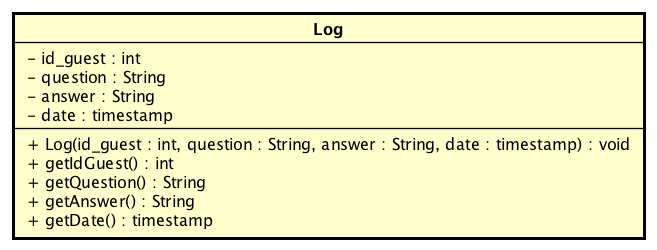
\includegraphics[scale=0.7]{Architettura/Front-End/Models/Log.png}
		\caption{Schema del componente \texttt{Models :: Log}}
	\end{figure}

		\subparagraph{Descrizione}: Rappresenta un log e ne contiene tutte le informazioni necessarie alla presentazione del suo contenuto
		\subparagraph{Utilizzo}: Viene utilizzata per memorizzare i dati di un log
		\subparagraph{Attributi}:
		      \begin{itemize}
		      	\item \texttt{answer: string}:
		      	      Attributo che rappresenta la risposta legata ad un log.

		      	\item \texttt{date: string}:
		      	      Attributo che rappresenta la data legata ad un log.

		      	\item \texttt{id\_guest: int}:
		      	      Attributo che rappresenta l'id dell'ospite in un log.

		      	\item \texttt{question: string}:
		      	      Attributo che rappresenta la domanda legata ad un log.
		      \end{itemize}
		\subparagraph{Metodi}:
		      \begin{itemize}
		      	\item \texttt{getAnswer : string}
		      	      \subparagraph{Descrizione}:Funzione che permette di ottenere il testo della risposta legato ad un log

		      	\item \texttt{getDate : string}
		      	      \subparagraph{Descrizione}:Funzione che permette di ottenere la data legata ad un log

		      	\item \texttt{getDate : string}:
		      	      Getter del timestamp del log

		      	\item \texttt{getIdGuest : int}
		      	      \subparagraph{Descrizione}: Funzione che permette di ottenere l'id\_guest legato ad un log

		      	\item \texttt{getQuestion : string}
		      	      \subparagraph{Descrizione}: Funzione che permette di ottenere il testo della domanda legato ad un log

		      	\item \texttt{Log}:
		      	      \subparagraph{Descrizione}:Costruttore del modello Log
					\subparagraph{Argomenti}:
						\begin{itemize}
							\item \texttt{date : string}:
								Parametro che indica la data legata al log.
							\item \texttt{id\_guest : int}:
								Parametro che indica l'id\_guest legato al Log.
							\item \texttt{question : string}:
								Parametro che indica il testo della domanda legata al log.
						\end{itemize}
		      \end{itemize}

		\subparagraph{Relazioni con altre classi}:
		      \begin{itemize}
		      	\item \texttt{Front-End :: AdminPage :: AdminComponents :: ManageFirmsComponent :: ManageFirmsController}: Componente per la scelta degli oggetti di tipo Firm.
		      \end{itemize}

	\newpage
	\paragraph{\texttt{Models :: Question}}
	\acapo
	\begin{figure}[!h]
		\centering
		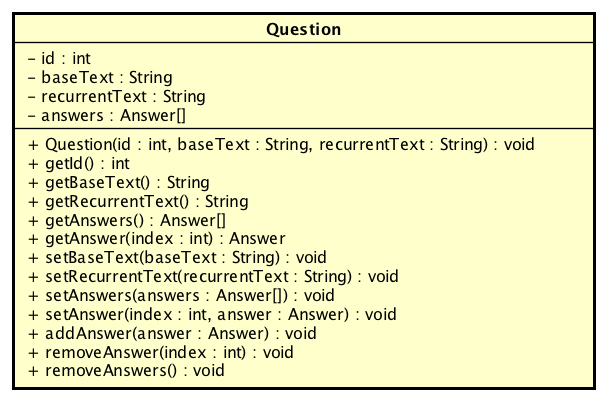
\includegraphics[scale=0.7]{Architettura/Front-End/Models/Question.png}
		\caption{Schema del componente \texttt{Models :: Question}}
	\end{figure}

		\subparagraph{Descrizione}: Rappresenta una domanda e ne contiene tutte le informazioni necessarie alla presentazione del suo contenuto
		\subparagraph{Utilizzo}: Viene utilizzata per memorizzare i dati di una domanda
		\subparagraph{Attributi}:
		      \begin{itemize}
		      	\item \texttt{answers: Answer[]}:
		      	      Attributo che rappresenta l'insieme delle risposte allegate ad una domanda.

		      	\item \texttt{baseText: string}:
		      	      Attributo che rappresenta il testo base di una domanda.

		      	\item \texttt{id: int}:
		      	      Attributo che rappresenta l'id di una domanda.

		      	\item \texttt{recurrentText: string}:
		      	      Attributo che rappresenta il testo ricorrente di una domanda.
		      \end{itemize}
		\subparagraph{Metodi}:
		      \begin{itemize}
		      	\item \texttt{addAnswer}
		      	      \subparagraph{Descrizione}:Aggiunge una risposta
		      	\subparagraph{Argomenti}:
		      	      \begin{itemize}
		      	      	\item \texttt{answer : Answer}:
		      	      	      Risposta.
		      	      \end{itemize}

		      	\item \texttt{getAnswer : Action}
		      	      \subparagraph{Descrizione}Ricerca di una riposta tramite indice
		      	\subparagraph{Argomenti}:
		      	      \begin{itemize}
		      	      	\item \texttt{index : int}:
		      	      	      Indice della risposta.
		      	      \end{itemize}

		      	\item \texttt{getAnswers : Answer[]}
		      	      \subparagraph{Descrizione}:Getter delle risposte

		      	\item \texttt{getBaseText : string}
		      	      \subparagraph{Descrizione}:Getter del testo base

		      	\item \texttt{getId : int}
		      	      \subparagraph{Descrizione}:Getter dell'ID della domanda

		      	\item \texttt{getRecurrentText : string}
		      	      \subparagraph{Descrizione}:Getter del testo ricorrente

		      	\item \texttt{Question}
		      	      \subparagraph{Descrizione}:Costruttore
					\subparagraph{Argomenti}:
						\begin{itemize}
							\item \texttt{id : int}:
								Id della domanda.
						\end{itemize}

		      	\item \texttt{removeAnswer}
		      	      \subparagraph{Descrizione}:Rimuove una domanda
					\subparagraph{Argomenti}:
						\begin{itemize}
							\item \texttt{index : int}:
								indice della domanda da rimuovere.
						\end{itemize}

		      	\item \texttt{removeAnswers}
		      	      \subparagraph{Descrizione}:Rimuove tutte le risposte

		      	\item \texttt{setAnswer}
		      	      \subparagraph{Descrizione}:Setter di una risposta

		      	\item \texttt{setAnswers}
		      	      \subparagraph{Descrizione}:Setter delle risposte

		      	\item \texttt{setBaseText}
		      	      \subparagraph{Descrizione}:Setter del testo base

		      	\item \texttt{setRecurrentText(recurrentText)}
		      	      \subparagraph{Descrizione}:Setter del testo ricorrente
					\subparagraph{Argomenti}:
						\begin{itemize}
							\item \texttt{recurrentText : string}:
								Testo ricorrente.
						\end{itemize}
		      \end{itemize}\vspace{0.5em}
		\subparagraph{Relazioni con altre classi}:
		      \begin{itemize}
		      	\item \texttt{Front-End :: AdminPage :: AdminComponents :: ManageQuestionsComponent :: ManageQuestionsController}: Componente per le domande e interazioni.
		      \end{itemize}



\subsection{\texttt{Angular 2}}
\subparagraph{Informazioni sul package}
\begin{itemize}
	\item \textbf{Descrizione}: Package che si riferisce al componente esterno Angular 2 che si utilizza nell'architettura
\end{itemize}
\subsection{\texttt{APIGateway}}
\subparagraph{Informazioni sul package}
\begin{itemize}
	\item \textbf{Descrizione}: Package dedicato all'interfaccia REST
\end{itemize}
\newpage
\subsection{\texttt{Back-End}}
\begin{figure}[!h]
	\centering
	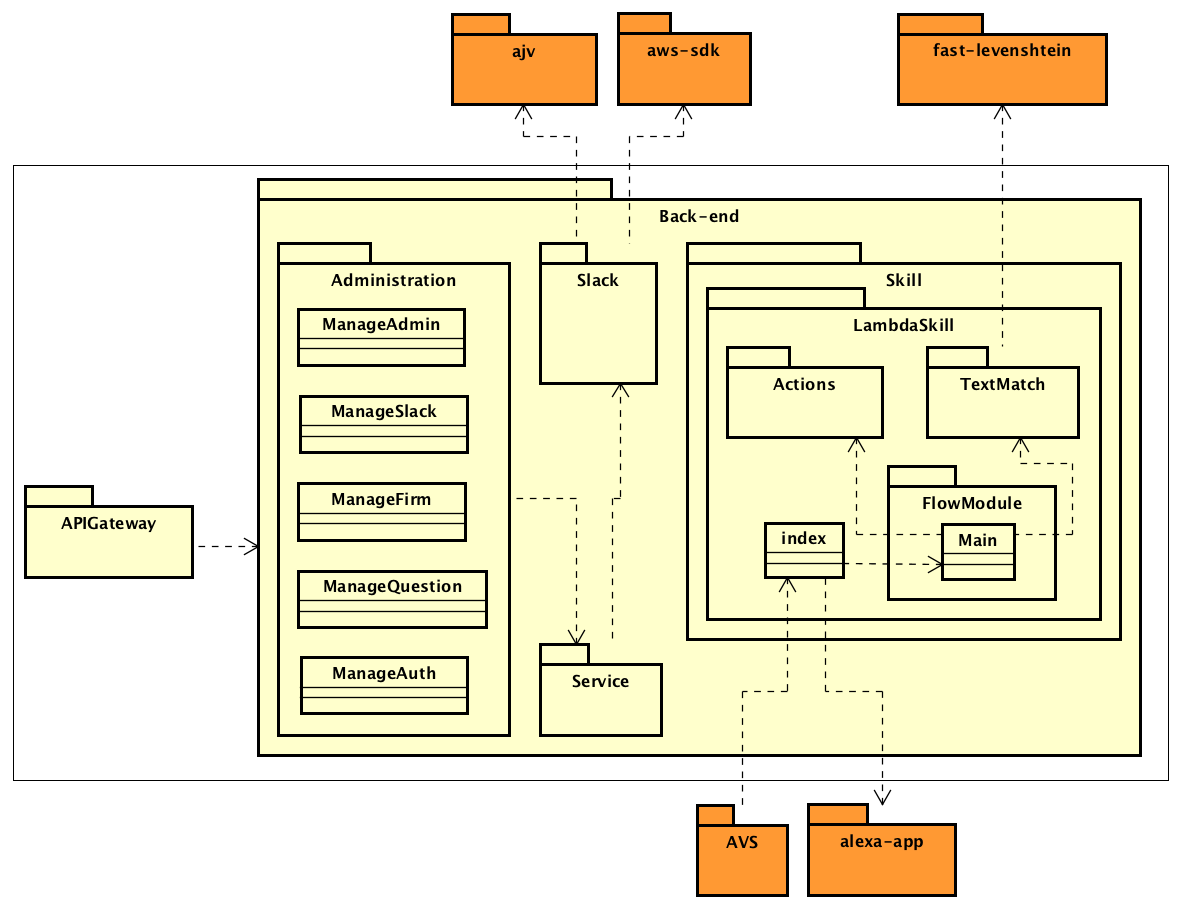
\includegraphics[width=\textwidth]{Architettura/Back-end.png}
	\caption{Schema del componente \texttt{Back-End}}
\end{figure}
\subparagraph{Informazioni sul package}
\begin{itemize}
	\item \textbf{Descrizione}: Package che contiene tutti i package dedicati alla parte logica dell'applicazione\item \textbf{Package contenuti}:
	      \begin{itemize}
	      	\item Back-End :: Administration: Package che contiene tutte le funzionalità che un Admin ed un SuperAdmin possono avere;
	      	\item Back-End :: Service: Package che gestisce tutti i servizi disponibili nell'applicazione;
	      	\item Back-End :: Slack: package per la gestione di Slack;
	      	\item Back-End :: Skill: package per la Skill di Alexa.
	      \end{itemize}
\end{itemize}
\subsubsection{\texttt{Back-End :: Administration}}
\subparagraph{Descrizione}: Package che contiene le possibili metodi delegati alla risposta alle interazioni del Front-End.\\
La classe contenuta in questo package non è ancora stata ben definita, poiché un inserimento più ampio di azioni è previsto come requisito opzionale, quindi la definizione specifica di questa classe viene rimandata dopo la codifica dei requisiti obbligatori.
\subsubsection{\texttt{Back-End :: Administration :: ManageAdmin}}
\subparagraph{Descrizione}: Package per la gestione degli amministratori.

\paragraph{\texttt{Back-End :: Administration :: ManageAdmin :: index}}
\subparagraph{Descrizione}: Classe handler per la gestione degli amministratori
\subparagraph{Dipendenze}:
\begin{itemize}
	\item	{Back-End :: Service :: AdminService}
\end{itemize}
\subparagraph{Costanti}:
\begin{itemize}
	\item \texttt{adminService}: modulo AdminService
\end{itemize}
\subparagraph{Metodi}:
\begin{itemize}
	\item \texttt{action}
	      \subparagraph{Descrizione}: Funzione che mediante uno switch dovrà suddividere le azioni da svolgere a seconda delle risorse richieste e metodi utilizzati per la chiamata alle API, da consultare le precedenti tabelle.
	\item \texttt{done}
	      \subparagraph{Descrizione}: Funzione che se "err" è null richiama la callback tornando un API trame. In caso di errore verrà impostato la risposta http a 400, in caso contrario a 200.
	      \subparagraph{Parametri}:
	      \begin{itemize}
	      	\item \texttt{err : object}:contiene l'errore {Error:"",TypeError:""} se avvenuto, null altrimenti;
	      	\item \texttt{res : object}:contiene il risultato se l'operazione è riuscita, null altrimenti;
	      \end{itemize}
	\item \texttt{handler}
	      \begin{itemize}
	      	\item \texttt{event : object}: evento dell'APIGateway;
	      	\item \texttt{context : object}: contesto di chiamata della funzione;
	      	\item \texttt{callback : function}: funzione di chiusura chiamata API da richiamare alla fine passando come parametro la risposta.
	      \end{itemize}
\end{itemize}
\subsubsection{\texttt{Back-End :: Administration :: ManageAuth}}
\subparagraph{Descrizione}: Package per la gestione dell'autenticazione.

\paragraph{\texttt{Back-End :: Administration :: ManageAuth :: index}}
\subparagraph{Descrizione}: Classe handler per la gestione dell'autenticazione.
\subparagraph{Dipendenze}:
\begin{itemize}
	\item \texttt{Back-End :: Service :: AuthService}
	\item	\texttt{Back-End :: Service :: AdminService}
\end{itemize}
\subparagraph{Costanti}:
\begin{itemize}
	\item \texttt{authService}: modulo AuthService
	\item \texttt{adminService}: modulo AdminService
\end{itemize}
\subparagraph{Metodi}:
\begin{itemize}
	\item \texttt{action}
	      \subparagraph{Descrizione}: Funzione che mediante uno switch dovrà suddividere le azioni da svolgere a seconda delle risorse richieste e metodi utilizzati per la chiamata alle API, da consultare le precedenti tabelle.
	\item \texttt{done}
	      \subparagraph{Descrizione}: Funzione che se "err" è null richiama la callback tornando un API trame. In caso di errore verrà impostato la risposta http a 400, in caso contrario a 200.
	      \subparagraph{Parametri}:
	      \begin{itemize}
	      	\item \texttt{err : object}:contiene l'errore {Error:"",TypeError:""} se avvenuto, null altrimenti;
	      	\item \texttt{res : object}:contiene il risultato se l'operazione è riuscita, null altrimenti;
	      \end{itemize}
	\item \texttt{handler}
	      \begin{itemize}
	      	\item \texttt{event : object}: evento dell'APIGateway;
	      	\item \texttt{context : object}: contesto di chiamata della funzione;
	      	\item \texttt{callback : function}: funzione di chiusura chiamata API da richiamare alla fine passando come parametro la risposta.
	      \end{itemize}
\end{itemize}
\subsubsection{\texttt{Back-End :: Administration :: ManageFirm}}
\subparagraph{Descrizione}: Package per la gestione delle informazioni sulle aziende e gli ospiti.

\paragraph{\texttt{Back-End :: Administration :: ManageFirm :: index}}
\subparagraph{Descrizione}: Classe handler per la gestione delle informazioni sulle aziende e gli ospiti.
\subparagraph{Dipendenze}:
\begin{itemize}
	\item \texttt{Back-End :: Service :: FirmService}
\end{itemize}
\subparagraph{Costanti}:
\begin{itemize}
	\item \texttt{firmSerivice}: modulo FirmService
\end{itemize}
\subparagraph{Metodi}:
\begin{itemize}
	\item \texttt{action}
	      \subparagraph{Descrizione}: Funzione che mediante uno switch dovrà suddividere le azioni da svolgere a seconda delle risorse richieste e metodi utilizzati per la chiamata alle API, da consultare le precedenti tabelle.
	\item \texttt{done}
	      \subparagraph{Descrizione}: Funzione che se "err" è null richiama la callback tornando un API trame. In caso di errore verrà impostato la risposta http a 400, in caso contrario a 200.
	      \subparagraph{Parametri}:
	      \begin{itemize}
	      	\item \texttt{err : object}:contiene l'errore {Error:"",TypeError:""} se avvenuto, null altrimenti;
	      	\item \texttt{res : object}:contiene il risultato se l'operazione è riuscita, null altrimenti;
	      \end{itemize}
	\item \texttt{handler}
	      \begin{itemize}
	      	\item \texttt{event : object}: evento dell'APIGateway;
	      	\item \texttt{context : object}: contesto di chiamata della funzione;
	      	\item \texttt{callback : function}: funzione di chiusura chiamata API da richiamare alla fine passando come parametro la risposta.
	      \end{itemize}
\end{itemize}


\subsubsection{\texttt{Back-End :: Administration :: ManageQuestion}}
\subparagraph{Descrizione}: Package per la gestione delle domande e delle risposte.

\paragraph{\texttt{Back-End :: Administration :: ManageQuestion :: index}}
\subparagraph{Descrizione}: Classe handler per la gestione delle domande e delle risposte.
\subparagraph{Dipendenze}:
\begin{itemize}
	\item \texttt{Back-End :: Service :: QuestionService}
\end{itemize}
\subparagraph{Costanti}:
\begin{itemize}
	\item \texttt{questionService}: modulo QuestionService
\end{itemize}
\subparagraph{Metodi}:
\begin{itemize}
	\item \texttt{action}
	      \subparagraph{Descrizione}: Funzione che mediante uno switch dovrà suddividere le azioni da svolgere a seconda delle risorse richieste e metodi utilizzati per la chiamata alle API, da consultare le precedenti tabelle.
	\item \texttt{done}
	      \subparagraph{Descrizione}: Funzione che se "err" è null richiama la callback tornando un API trame. In caso di errore verrà impostato la risposta http a 400, in caso contrario a 200.
	      \subparagraph{Parametri}:
	      \begin{itemize}
	      	\item \texttt{err : object}:contiene l'errore {Error:"",TypeError:""} se avvenuto, null altrimenti;
	      	\item \texttt{res : object}:contiene il risultato se l'operazione è riuscita, null altrimenti;
	      \end{itemize}
	\item \texttt{handler}
	      \begin{itemize}
	      	\item \texttt{event : object}: evento dell'APIGateway;
	      	\item \texttt{context : object}: contesto di chiamata della funzione;
	      	\item \texttt{callback : function}: funzione di chiusura chiamata API da richiamare alla fine passando come parametro la risposta.
	      \end{itemize}
\end{itemize}


\subsubsection{\texttt{Back-End :: Administration :: ManageSlack}}
\subparagraph{Descrizione}: Package per la gestione delle impostazioni dell'integrazione con Slack.

\paragraph{\texttt{Back-End :: Administration :: ManageSlack :: index}}
\subparagraph{Descrizione}: Classe handler per la gestione delle impostazioni dell'integrazione con Slack.
\subparagraph{Dipendenze}:
\begin{itemize}
	\item \texttt{Back-End :: Service :: SlackService :: InfoSlack}
\end{itemize}
\subparagraph{Costanti}:
\begin{itemize}
	\item \texttt{infoSlack}: modulo InfoSlack
\end{itemize}
\subparagraph{Metodi}:
\begin{itemize}
	\item \texttt{action}
	      \subparagraph{Descrizione}: Funzione che mediante uno switch dovrà suddividere le azioni da svolgere a seconda delle risorse richieste e metodi utilizzati per la chiamata alle API, da consultare le precedenti tabelle.
	\item \texttt{done}
	      \subparagraph{Descrizione}: Funzione che se "err" è null richiama la callback tornando un API trame. In caso di errore verrà impostato la risposta http a 400, in caso contrario a 200.
	      \subparagraph{Parametri}:
	      \begin{itemize}
	      	\item \texttt{err : object}:contiene l'errore {Error:"",TypeError:""} se avvenuto, null altrimenti;
	      	\item \texttt{res : object}:contiene il risultato se l'operazione è riuscita, null altrimenti;
	      \end{itemize}
	\item \texttt{handler}
	      \begin{itemize}
	      	\item \texttt{event : object}: evento dell'APIGateway;
	      	\item \texttt{context : object}: contesto di chiamata della funzione;
	      	\item \texttt{callback : function}: funzione di chiusura chiamata API da richiamare alla fine passando come parametro la risposta.
	      \end{itemize}
\end{itemize}



\newpage
\subsubsection{\texttt{Back-End :: Service}}
\begin{figure}[!h]
	\centering
	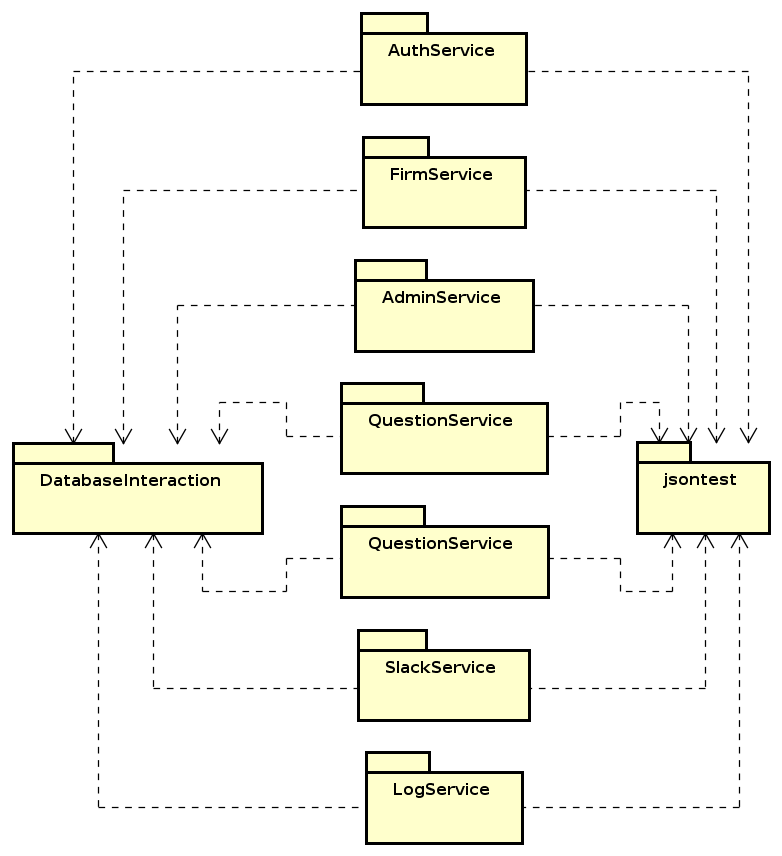
\includegraphics[scale=0.7]{Architettura/Back-End/Service/Service.png}
	\caption{Schema del componente \texttt{Back-End :: Service}}
\end{figure}
\subparagraph{Descrizione}: package che contiene tutte le classi dei service, ma è solo rappresentativo.
\newpage
\subsubsection{\texttt{Back-End :: Service :: AuthService}}
\begin{figure}[!h]
	\centering
	\includegraphics[scale=0.7]{Architettura/Back-End/Service/AuthService.png}
	\caption{Schema del componente \texttt{Back-End :: Service :: AuthService}}
\end{figure}
\subparagraph{Descrizione}: Package che contiene i servizi per l'autenticazione degli amministratori.
\paragraph{\texttt{Back-End :: Service :: AuthService :: AuthService}}
\subparagraph{Descrizione}: Modulo che fornisce i metodi per l'autenticazione degli amministratori.
\subparagraph{Dipendenze}:
\begin{itemize}
	\item \texttt{Back-End :: Service :: DatabaseInteraction}
	\item \texttt{Back-End :: Service :: TestJson}
\end{itemize}
\subparagraph{Costanti}:
\begin{itemize}
	\item \texttt{db}: modulo DatabaseInteraction
	\item \texttt{table}: Stringa contente il nome della tabella del db
	\item \texttt{crypto}: modulo crypto
	\item \texttt{jsontest}: modulo TestJson
\end{itemize}
\subparagraph{Metodi}:
\begin{itemize}
	\item \texttt{Login}:
	      \subparagraph{Descrizione}: funzione che passa username e password e restituisce in callback, err e res, dove res contiene l'amministratore ed err l'errore
	      \subparagraph{Parametri}:
	      \begin{itemize}
	      	\item \texttt{username : string}
	      	\item \texttt{password : string}
	      	\item \texttt{callback : function}:
	      \end{itemize}
	\item \texttt{Logout}: funzione che cancella il token dall'utente e restituisce in callback, err e res, dove res sarà sempre null ed err può contenere l'errore
	      \subparagraph{Descrizione}: Funzione per il login
	      \subparagraph{Parametri}:
	      \begin{itemize}
	      	\item \texttt{token : string}
	      	\item \texttt{username : string}
	      	\item \texttt{callback : function}
	      \end{itemize}
	\item \texttt{verifyLogin}: funzione che restituisce in callback, err e res, dove res contiene l'amministratore con il relativo token
	      \subparagraph{Descrizione}: Funzione per il login
	      \subparagraph{Parametri}:
	      \begin{itemize}
	      	\item \texttt{token : string}
	      	\item \texttt{callback : function}
	      \end{itemize}
	\item \texttt{passwordRecoveryToken}: funzione che restituisce in callback err e res
	      \subparagraph{Descrizione}: Funzione per il login
	      \subparagraph{Parametri}: \begin{itemize}
	\item \texttt{mail : string}
	\item \texttt{callback : function}
\end{itemize}
\item \texttt{validateAuth}: ritorna un {"validate":"","error":[]} e verifica l'attinenza al JSONSchema dell'oggetto Auth.
\subparagraph{Descrizione}: Funzione per il login
\subparagraph{Parametri}: \begin{itemize}
\item \texttt{obj : object}
\end{itemize}
\item \texttt{sendEmail}: funzione che restituisce in callback (err,res)
\subparagraph{Descrizione}: Funzione per il login
\subparagraph{Parametri}: \begin{itemize}
\item \texttt{token : string}
\item \texttt{callback : function}
\end{itemize}
\end{itemize}
\newpage
\subsubsection{\texttt{Back-End :: Service :: AdminService}}
\begin{figure}[!h]
	\centering
	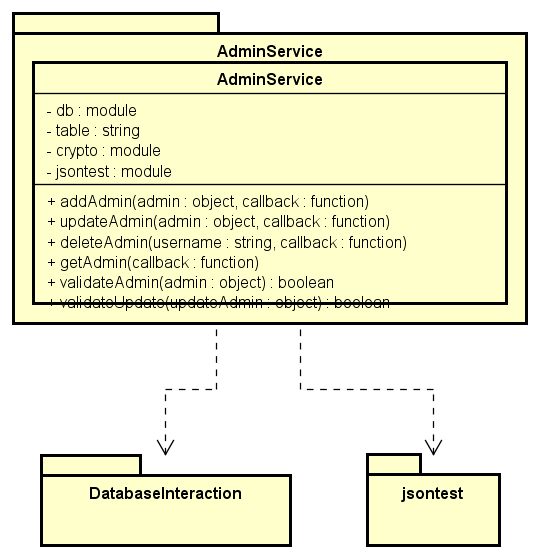
\includegraphics[scale=0.7]{Architettura/Back-End/Service/AdminService.png}
	\caption{Schema del componente \texttt{Back-End :: Service :: AdminService}}
\end{figure}
\subparagraph{Descrizione}: Package dedicato all'adminService

\paragraph{\texttt{Back-End :: Service :: AdminService :: AdminService}}
\subparagraph{Descrizione}: Modulo contenente i servizi rivolti all'admin
\subparagraph{Dipendenze}:
\begin{itemize}
	\item \texttt{Back-End :: Service :: DatabaseInteraction}
	\item \texttt{Back-End :: Service :: TestJson}
\end{itemize}
\subparagraph{Costanti}:
\begin{itemize}
	\item \texttt{db}: modulo DatabaseInteraction
	\item \texttt{table}: Stringa contente il nome della tabella del db
	\item \texttt{crypto}: modulo crypto
	\item \texttt{jsontest}: modulo TestJson
\end{itemize}
\subparagraph{Metodi}:\begin{itemize}
\item \texttt{addAdmin}:
\subparagraph{Descrizione}: funzione che inserisce nel database Admin. Restituisce in callback, err e res, e in res l'amministratore con quel username e password
\subparagraph{Parametri}: \begin{itemize}
\item \texttt{admin : object}
\item \texttt{callback : function}
\end{itemize}
\item \texttt{updateAdmin}:
\subparagraph{Descrizione}: funzione che aggiorna nel database l'admin. Restituisce in callback, err e res, e in res che contiene null.
\subparagraph{Parametri}: \begin{itemize}
\item \texttt{admin : object}
\item \texttt{callback : function}
\end{itemize}
\item \texttt{deleteAdmin}:
\subparagraph{Descrizione}: funzione cancella l'amministratore passato dal database. Restituisce in callback, err e res, e in res null
\subparagraph{Parametri}: \begin{itemize}
\item \texttt{username : string}
\item \texttt{callback : function}
\end{itemize}
\item \texttt{getAdmin}:
\subparagraph{Descrizione}: funzione che restituisce in callback, err e res, e in res tutti gli amministratori.
\subparagraph{Parametri}: \begin{itemize}
\item \texttt{callback : function}
\end{itemize}
\item \texttt{validateAdmin}:
\subparagraph{Descrizione}: ritorna un {"validate":"","error":[]} e verifica l'attinenza al JSONSchema dell'oggetto admin.
\subparagraph{Parametri}: \begin{itemize}
\item \texttt{admin : object}
\end{itemize}
\item \texttt{validateUpdate}:
\subparagraph{Descrizione}: ritorna un {"validate":"","error":[]} e verifica l'attinenza al JSONSchema dell'oggetto update.
\subparagraph{Parametri}: \begin{itemize}
\item \texttt{updateAdmin : object}
\end{itemize}
\end{itemize}
\newpage
\subsubsection{\texttt{Back-End :: Service :: SlackService}}
\begin{figure}[!h]
	\centering
	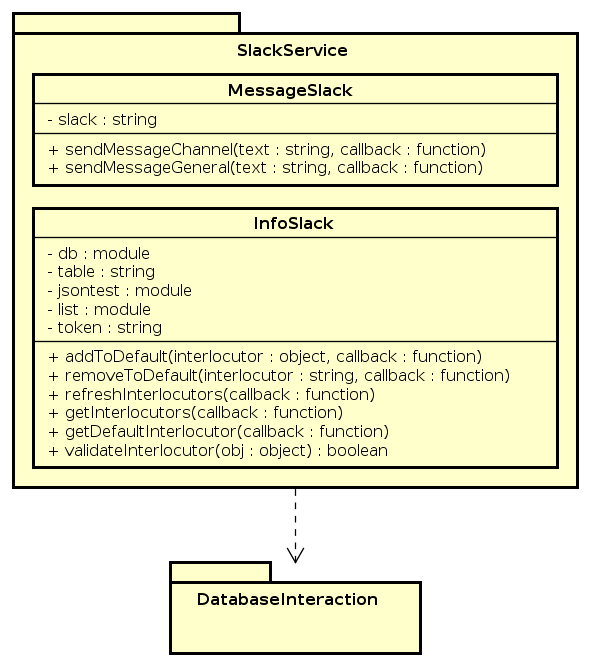
\includegraphics[scale=0.7]{Architettura/Back-End/Service/SlackService.png}
	\caption{Schema del componente \texttt{Back-End :: Service :: SlackService}}
\end{figure}
\subparagraph{Descrizione}: Pakage dedicato all'adminService

\paragraph{\texttt{Back-End :: Service :: SlackService :: InfoSlack}}
\subparagraph{Descrizione}: Modulo contenente i servizi rivolti all'admin
\subparagraph{Dipendenze}:
\begin{itemize}
	\item \texttt{Back-End :: Service :: DatabaseInteraction}
	\item \texttt{Back-End :: Service :: TestJson}
	\item \texttt{Back-End :: Slack :: Slack}
\end{itemize}
\subparagraph{Costanti}:
\begin{itemize}
	\item \texttt{db}: modulo DatabaseInteraction
	\item \texttt{table}: stringa contente il nome della tabella del db
	\item \texttt{list}: modulo
	\item \texttt{token}: stringa contenente il token di accesso a slack
	\item \texttt{jsontest}: modulo TestJson
\end{itemize}
\subparagraph{Metodi}:\begin{itemize}
\item \texttt{addToDefault}:
\subparagraph{Descrizione}: funzione che modifica l'interlocutor nel database impostando isDefault a false. Restituisce in callback, err e res, e in res null
\subparagraph{Parametri}: \begin{itemize}
\item \texttt{interlocutor : object}
\item \texttt{callback : function}
\end{itemize}
\item \texttt{removeToDefault}:
\subparagraph{Descrizione}: funzione che modifica l'interlocutor nel database impostando isDefault a false. Restituisce in callback, err e res, e in res null
\subparagraph{Parametri}: \begin{itemize}
\item \texttt{interlocutor : object}
\item \texttt{callback : function}
\end{itemize}
\item \texttt{refreshInterlocutors}:
\subparagraph{Descrizione}: funzione che sincronizza gli interlocutor tra il team di slack senza perdere le caratteristiche già presenti. Restituisce in callback, err e res, e in res null
\subparagraph{Parametri}: \begin{itemize}
\item \texttt{callback : function}
\end{itemize}
\item \texttt{getInterlocutors}:
\subparagraph{Descrizione}: funzione che restituisce in callback, err e res, e in res la lista degli interlocutori presenti nel database.
\subparagraph{Parametri}: \begin{itemize}
\item \texttt{callback : function}
\end{itemize}
\item \texttt{getDefaultInterlocutors}:
\subparagraph{Descrizione}: funzione che restituisce in callback, err e res, e in res la lista degli interlocutori con isDefault impostato a "true" presenti nel database.
\subparagraph{Parametri}: \begin{itemize}
\item \texttt{callback : function}
\end{itemize}
\item \texttt{validateInterlocutor}:
\subparagraph{Descrizione}: ritorna un {"validate":"","error":[]} e verifica l'attinenza al JSONSchema dell'oggetto interlocutor.
\subparagraph{Parametri}: \begin{itemize}
\item \texttt{obj : object}
\end{itemize}
\end{itemize}

\paragraph{\texttt{Back-End :: Service :: SlackService :: MessageSlack}}
\subparagraph{Descrizione}: Modulo contenente i servizi rivolti all'admin
\subparagraph{Dipendenze}:
\begin{itemize}
	\item \texttt{Back-End :: Slack :: Slack}
\end{itemize}
\subparagraph{Costanti}:
\begin{itemize}
	\item \texttt{slack}: modulo di slack
\end{itemize}
\subparagraph{Metodi}:\begin{itemize}
\item \texttt{SendMessageChannel}:
\subparagraph{Descrizione}: funzione che spedisce un messaggio contenente text in channel. Restituisce in callback, err e res, e in res null
\subparagraph{Parametri}: \begin{itemize}
\item \texttt{text : string}
\item \texttt{channel : string}
\item \texttt{callback : function}
\end{itemize}
\item \texttt{SendMessageGeneral}:
\subparagraph{Descrizione}: funzione che spedisce un messaggio contenente text in general. Restituisce in callback, err e res, e in res null
\subparagraph{Parametri}: \begin{itemize}
\item \texttt{text : string}
\item \texttt{callback : function}
\end{itemize}
\end{itemize}

\newpage
\subsubsection{\texttt{Back-End :: Service :: FirmService}}
\begin{figure}[!h]
	\centering
	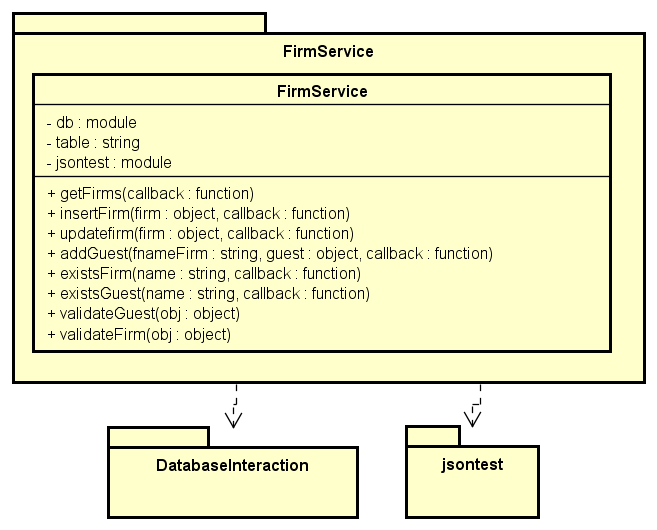
\includegraphics[scale=0.7]{Architettura/Back-End/Service/FirmService.png}
	\caption{Schema del componente \texttt{Back-End :: Service :: FirmService}}
\end{figure}

\subparagraph{Descrizione}: Pakage dedicato ai servizi riguardanti le firm

\paragraph{\texttt{Back-End :: Service :: FirmService :: FirmService}}
\subparagraph{Descrizione}: Modulo contenente i servizi rivolti all'admin
\subparagraph{Dipendenze}:
\begin{itemize}
	\item \texttt{Back-End :: Service :: DatabaseInteraction}
	\item \texttt{Back-End :: Service :: TestJson}
\end{itemize}
\subparagraph{Costanti}:
\begin{itemize}
	\item \texttt{db}: modulo DatabaseInteraction
	\item \texttt{table}: stringa contente il nome della tabella del database
	\item \texttt{jsontest}: modulo TestJson
\end{itemize}
\subparagraph{Metodi}:\begin{itemize}
\item \texttt{getFirms}:
\subparagraph{Descrizione}: funzione che restituisce in callback, err e res, e in res la lista delle firm contenute nel database
\subparagraph{Parametri}: \begin{itemize}
\item \texttt{callback : function}
\end{itemize}
\item \texttt{inserFirm}:
\subparagraph{Descrizione}: funzione che inserisce l'oggetto firm nel database. Restituisce in callback, err e res, e in res null
\subparagraph{Parametri}: \begin{itemize}
\item \texttt{interlocutor : object}
\item \texttt{callback : function}
\end{itemize}
\item \texttt{updateFirm}:
\subparagraph{Descrizione}: funzione che aggiorna l'oggetto firm nel database. Restituisce in callback, err e res, e in res null
\subparagraph{Parametri}: \begin{itemize}
\item \texttt{firm : object}
\item \texttt{callback : function}
\end{itemize}
\item \texttt{addGuest}:
\subparagraph{Descrizione}: :funzione che aggiunge l'oggetto guest sulla corrispettiva azienda nel database. Restituisce in callback, err e res, e in res null
\subparagraph{Parametri}: \begin{itemize}
\item \texttt{nameFirm : string}
\item \texttt{guest : object}
\item \texttt{callback : function}
\end{itemize}
\item \texttt{existsFirm}:
\subparagraph{Descrizione}: :funzione che verifica l'esistenza dell'oggetto firm nel database. Restituisce in callback, err e res, e in res un booleano
\subparagraph{Parametri}: \begin{itemize}
\item \texttt{name : string}
\item \texttt{callback : function}
\end{itemize}
\item \texttt{existsGuest}:
\subparagraph{Descrizione}: funzione che verifica l'esistenza dell'oggetto guest nel database. Restituisce in callback, err e res, e in res un booleano
\subparagraph{Parametri}: \begin{itemize}
\item \texttt{name : string}
\item \texttt{callback : function}
\end{itemize}
\item \texttt{validateGuest}:
\subparagraph{Descrizione}: ritorna un oggetto {"validate":"","error":[]} e verifica l'attinenza al JSONSchema dell'oggetto Guest.
\subparagraph{Parametri}: \begin{itemize}
\item \texttt{obj : object}
\end{itemize}
\item \texttt{validateFirm}:
\subparagraph{Descrizione}: ritorna un {"validate":"","error":[]}  e verifica l'attinenza al JSONSchema dell'oggetto Firm.
\subparagraph{Parametri}: \begin{itemize}
\item \texttt{obj : object}
\end{itemize}
\end{itemize}
\newpage

\subsubsection{\texttt{Back-End :: Service :: QuestionService}}
\begin{figure}[!h]
	\centering
	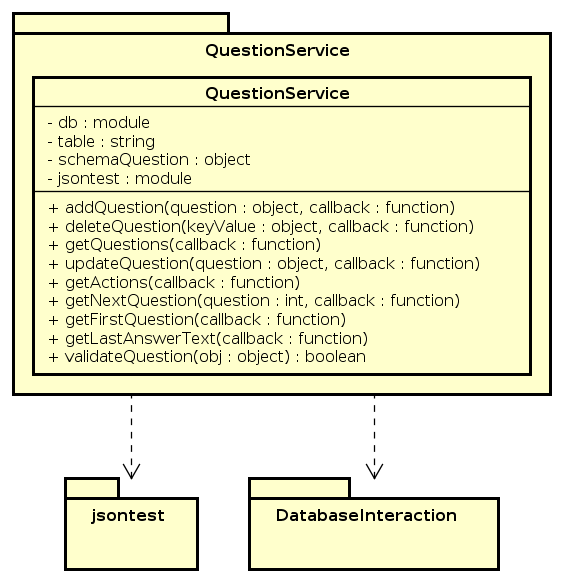
\includegraphics[scale=0.7]{Architettura/Back-End/Service/QuestionService.png}
	\caption{Schema del componente \texttt{Back-End :: Service :: QuestionService}}
\end{figure}

\subparagraph{Descrizione}:Pakage dedicato ai servizi riguardanti le firm

\paragraph{\texttt{Back-End :: Service :: QuestionService :: QuestionService}}
\subparagraph{Descrizione}: Modulo contenente i servizi rivolti all'admin
\subparagraph{Dipendenze}:
\begin{itemize}
	\item \texttt{Back-End :: Service :: DatabaseInteraction}
	\item \texttt{Back-End :: Service :: TestJson}
\end{itemize}
\subparagraph{Costanti}:
\begin{itemize}
	\item \texttt{db}: modulo DatabaseInteraction
	\item \texttt{table}: stringa contente il nome della tabella del database
	\item \texttt{schemaQuestion}: oggetto che contiene il JSONSchema di question
	\item \texttt{jsontest}: modulo TestJson
\end{itemize}
\subparagraph{Metodi}:\begin{itemize}
\item \texttt{getQuestions}:
\subparagraph{Descrizione}:funzione che restituisce in callback, err e res, e in res la lista delle question contenute nel database
\subparagraph{Parametri}:
\begin{itemize}
	\item \texttt{callback : function}
\end{itemize}
\item \texttt{addQuestion}:
\subparagraph{Descrizione}:funzione che inserisce l'oggetto firm nel database. Restituisce in callback, err e res, e in res null
\subparagraph{Parametri}:
\begin{itemize}
	\item \texttt{question : object}
	\item \texttt{callback : function}
\end{itemize}
\item \texttt{deleteQuestion}:
\subparagraph{Descrizione}:funzione che elimina l'oggetto firm nel database. Restituisce in callback, err e res, e in res null
\subparagraph{Parametri}:
\begin{itemize}
	\item \texttt{keyValue : object}
	\item \texttt{callback : function}
\end{itemize}
\item \texttt{updateQuestion}:
\subparagraph{Descrizione}:funzione che inserisce l'oggetto firm nel database. Restituisce in callback, err e res, e in res null
\subparagraph{Parametri}:
\begin{itemize}
	\item \texttt{question : object}
	\item \texttt{callback : function}
\end{itemize}
\item \texttt{getActions}:
\subparagraph{Descrizione}:funzione che restituisce in callback, err e res, e in res la lista delle Action contenute nel database
\subparagraph{Parametri}:
\begin{itemize}
	\item \texttt{callback : function}
\end{itemize}
\item \texttt{deleteAction}:
\subparagraph{Descrizione}:funzione che restituisce in callback, err e res, e in res null, ed elimina la action 
\subparagraph{Parametri}:
\begin{itemize}
	\item \texttt{obj : object}
	\item \texttt{callback : function}
\end{itemize}
\item \texttt{getNextQuestions}:
\subparagraph{Descrizione}:funzione che restituisce in callback, err e res, e in res la  question successiva contenuta nel database rispetto a quella di chiave "question"
\subparagraph{Parametri}:
\begin{itemize}
	\item \texttt{question : int}
	\item \texttt{callback : function}
\end{itemize}
\item \texttt{getFirstQuestions}:
\subparagraph{Descrizione}:funzione che restituisce in callback, err e res, e in res l'ultima question contenute nel database
\subparagraph{Parametri}:
\begin{itemize}
	\item \texttt{callback : function}
\end{itemize}
\item \texttt{validateQuestion}:
\subparagraph{Descrizione}:ritorna un {"validate":"","error":[]}  e verifica l'attinenza al JSONSchema dell'oggetto Question.
\subparagraph{Parametri}:
\begin{itemize}
	\item \texttt{obj : object}
\end{itemize}
\end{itemize}
\newpage
\subsubsection{\texttt{Back-End :: Service :: LogService}}
\begin{figure}[!h]
	\centering
	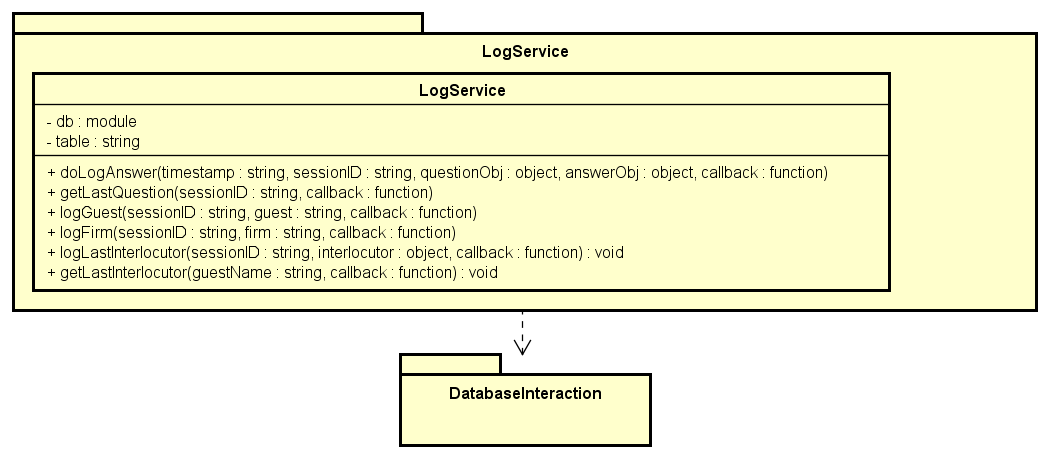
\includegraphics[width=\textwidth]{Architettura/Back-End/Service/LogService.png}
	\caption{Schema del componente \texttt{Back-End :: Service :: LogService}}
\end{figure}

\subparagraph{Descrizione}:Pakage dedicato ai servizi riguardanti i log effettuati da Alexa

\paragraph{\texttt{Back-End :: Service :: LogService :: LogService}}
\subparagraph{Descrizione}: Modulo contenente i servizi rivolti al logging della conversazione
\subparagraph{Dipendenze}:
\begin{itemize}
	\item \texttt{Back-End :: Service :: DatabaseInteraction}
\end{itemize}
\subparagraph{Costanti}:
\begin{itemize}
	\item \texttt{db}: modulo DatabaseInteraction
	\item \texttt{table}: stringa contente il nome della tabella del database
\end{itemize}
\subparagraph{Metodi}:
\begin{itemize}
\item \texttt{doLogAnswer}:
	\subparagraph{Descrizione}:funzione inserisce nel database l'oggetto Questionobj e QuestionAnswer incapsulati in un oggetto contenente una lista della conversazione "logg" e il sessionID. Restituisce in callback, err e res, e in res null
	\subparagraph{Parametri}:
	\begin{itemize}
		\item \texttt{timestamp : string}
		\item \texttt{sessionID : string}
		\item \texttt{questionObj : object}
		\item \texttt{questionObj : object}
		\item \texttt{callback : function}
	\end{itemize}
\item \texttt{getLastQuestion}:
	\subparagraph{Descrizione}:
	\subparagraph{Parametri}:
	\begin{itemize}
		\item \texttt{sessionID : string}
		\item \texttt{callback : function}

	\end{itemize}
\item \texttt{logGuest}:
	\subparagraph{Descrizione}:Permette di loggare il guest della sessione
	\subparagraph{Parametri}:
	\begin{itemize}
		\item \texttt{sessionID : string}
		\item \texttt{guest : string}
		\item \texttt{callback : function}

	\end{itemize}
\item \texttt{logFirm}:
	\subparagraph{Descrizione}:Permette di loggare la firm dell'ospite della sessione
	\subparagraph{Parametri}:
	\begin{itemize}
		\item \texttt{sessionID : string}
		\item \texttt{firm : string}
		\item \texttt{callback : function}

	\end{itemize}
\item \texttt{logLastInterlocutor}:
	\subparagraph{Descrizione}: permette di salvare l'interlocutore richiesto
	\subparagraph{Parametri}:
	\begin{itemize}
		\item \texttt{sessionID : string}
		\item \texttt{interlocutor : object}
		\item \texttt{callback : function}

	\end{itemize}
\item \texttt{getLastInterlocutor}:
	\subparagraph{Descrizione}: permette di tornare l'interlocutore richiesto in una sessione
	\subparagraph{Parametri}:
	\begin{itemize}
		\item \texttt{guestName : string}
		\item \texttt{callback : function}

	\end{itemize}

\item \texttt{getRecentGuest}:
	\subparagraph{Descrizione}: permette di salvare il guest di quella sessione
	\subparagraph{Parametri}:
	\begin{itemize}
		\item \texttt{firmName : string}
		\item \texttt{sessionId : string}
		\item \texttt{callback : function}
	\end{itemize}


\end{itemize}

\newpage
\subsubsection{\texttt{Back-End :: Service :: DatabaseInteraction}}
\begin{figure}[!h]
	\centering
	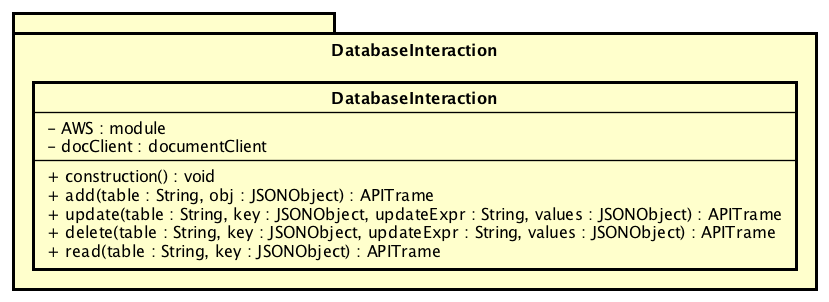
\includegraphics[width=\textwidth]{Architettura/Back-End/Service/DatabaseInteraction.png}
	\caption{Schema del componente \texttt{Back-End :: Service :: DatabaseInteraction}}
\end{figure}

\subparagraph{Descrizione}:Pakage dedicato ai servizi riguardanti i log effettuati da Alexa

\paragraph{\texttt{Back-End :: Service :: DatabaseInteraction :: DatabaseInteraction}}
\subparagraph{Descrizione}: Modulo contenente i servizi rivolti allo logging della conversazione
\subparagraph{Dipendenze}:
\begin{itemize}
	\item \texttt{AWS-sdk}
\end{itemize}
\subparagraph{Costanti}:
\begin{itemize}
	\item \texttt{AWS}: modulo AWS-sdk
	\item \texttt{config}: oggetto contenente le chiavi per l'accesso a DynamoDB
	\item \texttt{docClient}: oggetto per l'interrogazione del database DynamoDB
\end{itemize}
\subparagraph{Metodi}:\begin{itemize}
\item \texttt{insert}:
\subparagraph{Descrizione}: Inserisce l'oggetto nella "table" di DynamoDB attraverso le sdk e ci passa callback.
\subparagraph{Parametri}:
\begin{itemize}
	\item \texttt{table : string}
	\item \texttt{sessionID : object}
	\item \texttt{callback : function}
\end{itemize}
\item \texttt{update}:
\subparagraph{Descrizione}: Aggiorna l'oggetto con chiave "key" nella "table" di DynamoDB attraverso le sdk e ci passa callback.
\subparagraph{Parametri}:
\begin{itemize}
	\item \texttt{table : string}
	\item \texttt{key : object}
	\item \texttt{updateExpression : string}
	\item \texttt{replace : object}
	\item \texttt{callback : function}
\end{itemize}

\item \texttt{remove}:
\subparagraph{Descrizione}: rimuove l'oggetto con chiave "key" nella "table" di DynamoDB attraverso le sdk e ci passa callback.
\subparagraph{Parametri}:
\begin{itemize}
	\item \texttt{table : string}
	\item \texttt{key : object}
	\item \texttt{callback : function}
\end{itemize}

\item \texttt{read}:
\subparagraph{Descrizione}: Esegue la lettura dell'oggetto con chiave "key" nella "table" di DynamoDB attraverso le sdk e ci passa callback.
\subparagraph{Parametri}:
\begin{itemize}
	\item \texttt{table : string}
	\item \texttt{key : object}
	\item \texttt{callback : function}
\end{itemize}

\item \texttt{query}:
\subparagraph{Descrizione}: Esegue la lettura di tutti gli oggetti rispettanti la filter expression con i valori "attribute value" nella "table" di DynamoDB attraverso le sdk e ci passa callback.
\subparagraph{Parametri}:
\begin{itemize}
	\item \texttt{table : string}
	\item \texttt{filterExpression : string}
	\item \texttt{ExpressionAttributeValue : object}
	\item \texttt{callback : function}
\end{itemize}

\item \texttt{queryProp}:
\subparagraph{Descrizione}: Esegue la lettura delle "proprieties" di tutti gli oggetti rispettanti la filter expression con i valori "attribute value" nella "table" di DynamoDB attraverso le sdk e ci passa callback.
\subparagraph{Parametri}:
\begin{itemize}
	\item \texttt{table : string}
	\item \texttt{proprieties : string}
	\item \texttt{filterExpression : string}
	\item \texttt{ExpressionAttributeValue : object}
	\item \texttt{callback : function}
\end{itemize}

\item \texttt{readProp}:
\subparagraph{Descrizione}: Esegue la lettura delle proprietà dell'oggetto con chiave "key" nella "table" di DynamoDB attraverso le sdk e ci passa callback.
\subparagraph{Parametri}:
\begin{itemize}
	\item \texttt{table : string}
	\item \texttt{key : object}
	\item \texttt{properties : string}
	\item \texttt{callback : function}
\end{itemize}

\item \texttt{ConditionUpdate}:
\subparagraph{Descrizione}: Aggiorna l'oggetto con chiave "key" nella "table" di DynamoDB attraverso le sdk e ci passa callback.
\subparagraph{Parametri}:
\begin{itemize}
	\item \texttt{table : string}
	\item \texttt{key : object}
	\item \texttt{updateExpression : string}
	\item \texttt{condition : string}
	\item \texttt{replace : object}
	\item \texttt{callback : function}
\end{itemize}

\end{itemize}


\subsubsection{\texttt{Back-End :: JsonTest}}
\subparagraph{Descrizione}:Package dedicato ai servizi riguardanti i log effettuati da Alexa

\paragraph{\texttt{Back-End :: Service :: JsonTest :: TestJson}}
\subparagraph{Descrizione}: Modulo contenente i servizi rivolti alla validazione di un oggetto rispettivamente ad un JSONSchema.
\subparagraph{Dipendenze}:
\begin{itemize}
	\item \texttt{Ajv.js}
\end{itemize}
\subparagraph{Costanti}:
\begin{itemize}
	\item \texttt{Ajv}: modulo Ajv
\end{itemize}
\subparagraph{Metodi}:\begin{itemize}
\item \texttt{test}:
\subparagraph{Descrizione}: Controlla l'attinenza dell'oggetto obj allo JSONSchema utilizzando la libreria Ajv e tornando {"valid":false,"errors":array} in caso di errore con errors gli errori identificati, {"valid":true} in caso di attinenza.
\subparagraph{Parametri}:
\begin{itemize}
	\item \texttt{schema : object}
	\item \texttt{obj : object}
\end{itemize}
\end{itemize}

\newpage
\subsubsection{\texttt{Back-End :: Slack}}
\begin{figure}[!h]
	\centering
	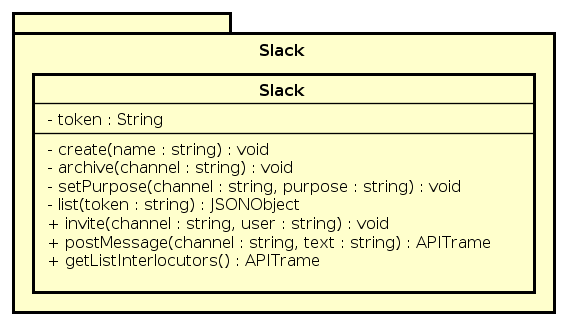
\includegraphics[scale=0.7]{Architettura/Back-End/Slack.png}
	\caption{Schema del componente \texttt{Back-End :: Slack}}
\end{figure}
\subparagraph{Descrizione}: Package che contiene le possibili metodi delegati alla risposta alle interazioni del Front-End.\\
La classe contenuta in questo package non è ancora stata ben definita, poiché un inserimento più ampio di azioni è previsto come requisito opzionale, quindi la definizione specifica di questa classe viene rimandata dopo la codifica dei requisiti obbligatori.

\paragraph{\texttt{Back-End :: Slack :: createChannel}}
\subparagraph{Descrizione}: Modulo per creare un canale in Slack
\subparagraph{Dipendenze}:
\begin{itemize}
	\item \texttt{querystring};
	\item \texttt{https}.
\end{itemize}
\subparagraph{Metodi}:
\begin{itemize}
	\item \texttt{createChannel}
	      \subparagraph{Descrizione}: Metodo per la creazione di un canale Slack
	      \subparagraph{Parametri}:
	      \begin{itemize}
	      	\item \texttt{token};
	      	\item \texttt{name};
	      	\item \texttt{callback}.
	      \end{itemize}
	      \subparagraph{Ritorno}: Utilizzando la callback, il metodo restituisce la risposta dell'API o un errore.
\end{itemize}

\paragraph{\texttt{Back-End :: Slack :: channelList}}
\subparagraph{Descrizione}: Modulo per ottenere la lista dei canali di Slack
\subparagraph{Dipendenze}:
\begin{itemize}
	\item \texttt{querystring};
	\item \texttt{https}.
\end{itemize}
\subparagraph{Metodi}:
\begin{itemize}
	\item \texttt{getChannelsList}
	      \subparagraph{Descrizione}: Metodo per ottenere la lista dei canali Slack
	      \subparagraph{Parametri}:
	      \begin{itemize}
	      	\item \texttt{token};
	      	\item \texttt{callback}.
	      \end{itemize}
	      \subparagraph{Ritorno}: Utilizzando la callback, il metodo restituisce la risposta dell'API o un errore.
\end{itemize}

\paragraph{\texttt{Back-End :: Slack :: invite}}
\subparagraph{Descrizione}: Modulo per invitare un interlocutore in un canale Slack
\subparagraph{dipendenze}:
\begin{itemize}
	\item \texttt{querystring};
	\item \texttt{https}.
\end{itemize}
\subparagraph{Metodi}:
\begin{itemize}
	\item \texttt{invite}
	      \subparagraph{Descrizione}: Metodo per invitare un utente Slack in un canale.
	      \subparagraph{Parametri}:
	      \begin{itemize}
	      	\item \texttt{token};
	      	\item \texttt{channelID};
	      	\item \texttt{userID};
	      	\item \texttt{callback}.
	      \end{itemize}
	      \subparagraph{Ritorno}: Utilizzando la callback, il metodo restituisce la risposta dell'API o un errore.
\end{itemize}

\paragraph{\texttt{Back-End :: Slack :: NameID}}
\subparagraph{Descrizione}: Modulo per trovare il valore corrispondente tra username dell'interlocutore e ID utente
\subparagraph{Dipendenze}:
\begin{itemize}
	\item \texttt{Back-End :: Slack :: ChannelList};
	\item \texttt{https}.
\end{itemize}
\subparagraph{Metodi}:
\begin{itemize}
	\item \texttt{name2ID}
	      \subparagraph{Descrizione}: Metodo per ottenere l'ID di un utente Slack dato il suo nome.
	      \subparagraph{Parametri}:
	      \begin{itemize}
	      	\item \texttt{token};
	      	\item \texttt{name};
	      	\item \texttt{callback}.
	      \end{itemize}
	      \subparagraph{Ritorno}: Utilizzando la callback, il metodo restituisce il nome dell'utente o un errore.
	\item \texttt{ID2name}
	      \subparagraph{Descrizione}: Metodo per ottenere il nome di un utente Slack dato il suo ID.
	      \subparagraph{Parametri}:
	      \begin{itemize}
	      	\item \texttt{token};
	      	\item \texttt{ID};
	      	\item \texttt{callback}.
	      \end{itemize}
	      \subparagraph{Ritorno}: Utilizzando la callback, il metodo restituisce l'ID dell'utente o un errore.
\end{itemize}

\paragraph{\texttt{Back-End :: Slack :: postMessage}}
\subparagraph{Descrizione}: Modulo per inviare messaggi ad un canale Slack
\subparagraph{Dipendenze}:
\begin{itemize}
	\item \texttt{https};
	\item \texttt{querystring};
	\item \texttt{Back-End :: Slack :: ChannelList};
	\item \texttt{Back-End :: Slack :: createChannel};
	\item \texttt{Back-End :: Slack :: NameID};
	\item \texttt{Back-End :: Slack :: unarchive};
	\item \texttt{Back-End :: Slack :: invite};
	\item \texttt{Back-End :: Slack :: setPurpose}.
\end{itemize}
\subparagraph{Metodi}:
\begin{itemize}
	\item \texttt{postMessage}
	      \subparagraph{Descrizione}: Metodo per inviare un messaggio ad un dato canale. Se il canale non esiste viene creato e vengono invitati gli utenti di default impostati dagli amministratori. Se il canale è archiviato questo viene disarchiviato e vengono invitati gli utenti di default.
	      \subparagraph{Parametri}:
	      \begin{itemize}
	      	\item \texttt{token};
	      	\item \texttt{channelName};
	      	\item \texttt{text};
	      	\item \texttt{callback}.
	      \end{itemize}
	      \subparagraph{Ritorno}: Utilizzando la callback, il metodo restituisce l'ID dell'utente o un errore.
\end{itemize}

\paragraph{\texttt{Back-End :: Slack :: setPurpose}}
\subparagraph{Descrizione}: Modulo per impostare lo scopo di un canale Slack.
\subparagraph{Dipendenze}:
\begin{itemize}
	\item \texttt{https};
	\item \texttt{querystring};
	\item \texttt{Back-End :: Slack :: NameID}.
\end{itemize}
\subparagraph{Metodi}:
\begin{itemize}
	\item \texttt{setPurpose}
	      \subparagraph{Descrizione}: Metodo per impostare lo scopo di un canale Slack.
	      \subparagraph{Parametri}:
	      \begin{itemize}
	      	\item \texttt{token};
	      	\item \texttt{channelID};
	      	\item \texttt{callback}.
	      \end{itemize}
	      \subparagraph{Ritorno}: Utilizzando la callback, il metodo restituisce la risposta dell'API o un errore.
\end{itemize}

\paragraph{\texttt{Back-End :: Slack :: unarchive}}
\subparagraph{Descrizione}: Modulo per dearchiviare un canale Slack che è stato archiviato.
\subparagraph{Dipendenze}:
\begin{itemize}
	\item \texttt{https};
	\item \texttt{querystring}.
\end{itemize}
\subparagraph{Metodi}:
\begin{itemize}
	\item \texttt{unarchiveChannelByID}
	      \subparagraph{Descrizione}: Metodo per dearchiviare un canale Slack.
	      \subparagraph{Parametri}:
	      \begin{itemize}
	      	\item \texttt{token};
	      	\item \texttt{channelID};
	      	\item \texttt{callbackData}.
	      \end{itemize}
	      \subparagraph{Ritorno}: Utilizzando la callback, il metodo restituisce la risposta dell'API o un errore.
\end{itemize}

\paragraph{\texttt{Back-End :: Slack :: userList}}
\subparagraph{Descrizione}: Modulo per ottenere la lista degli utenti di Slack
\subparagraph{Dipendenze}:
\begin{itemize}
	\item \texttt{https};
	\item \texttt{querystring}.
\end{itemize}
\subparagraph{Metodi}:
\begin{itemize}
	\item \texttt{userList}
	      \subparagraph{Descrizione}: Metodo per ottenere la lista degli utenti di Slack
	      \subparagraph{Parametri}:
	      \begin{itemize}
	      	\item \texttt{token};
	      	\item \texttt{callbackData}.
	      \end{itemize}
	      \subparagraph{Ritorno}: Utilizzando la callback, il metodo restituisce la risposta dell'API o un errore.
\end{itemize}

\newpage

\subsubsection{\texttt{Back-End :: Skill}}
\begin{figure}[!h]
	\centering
	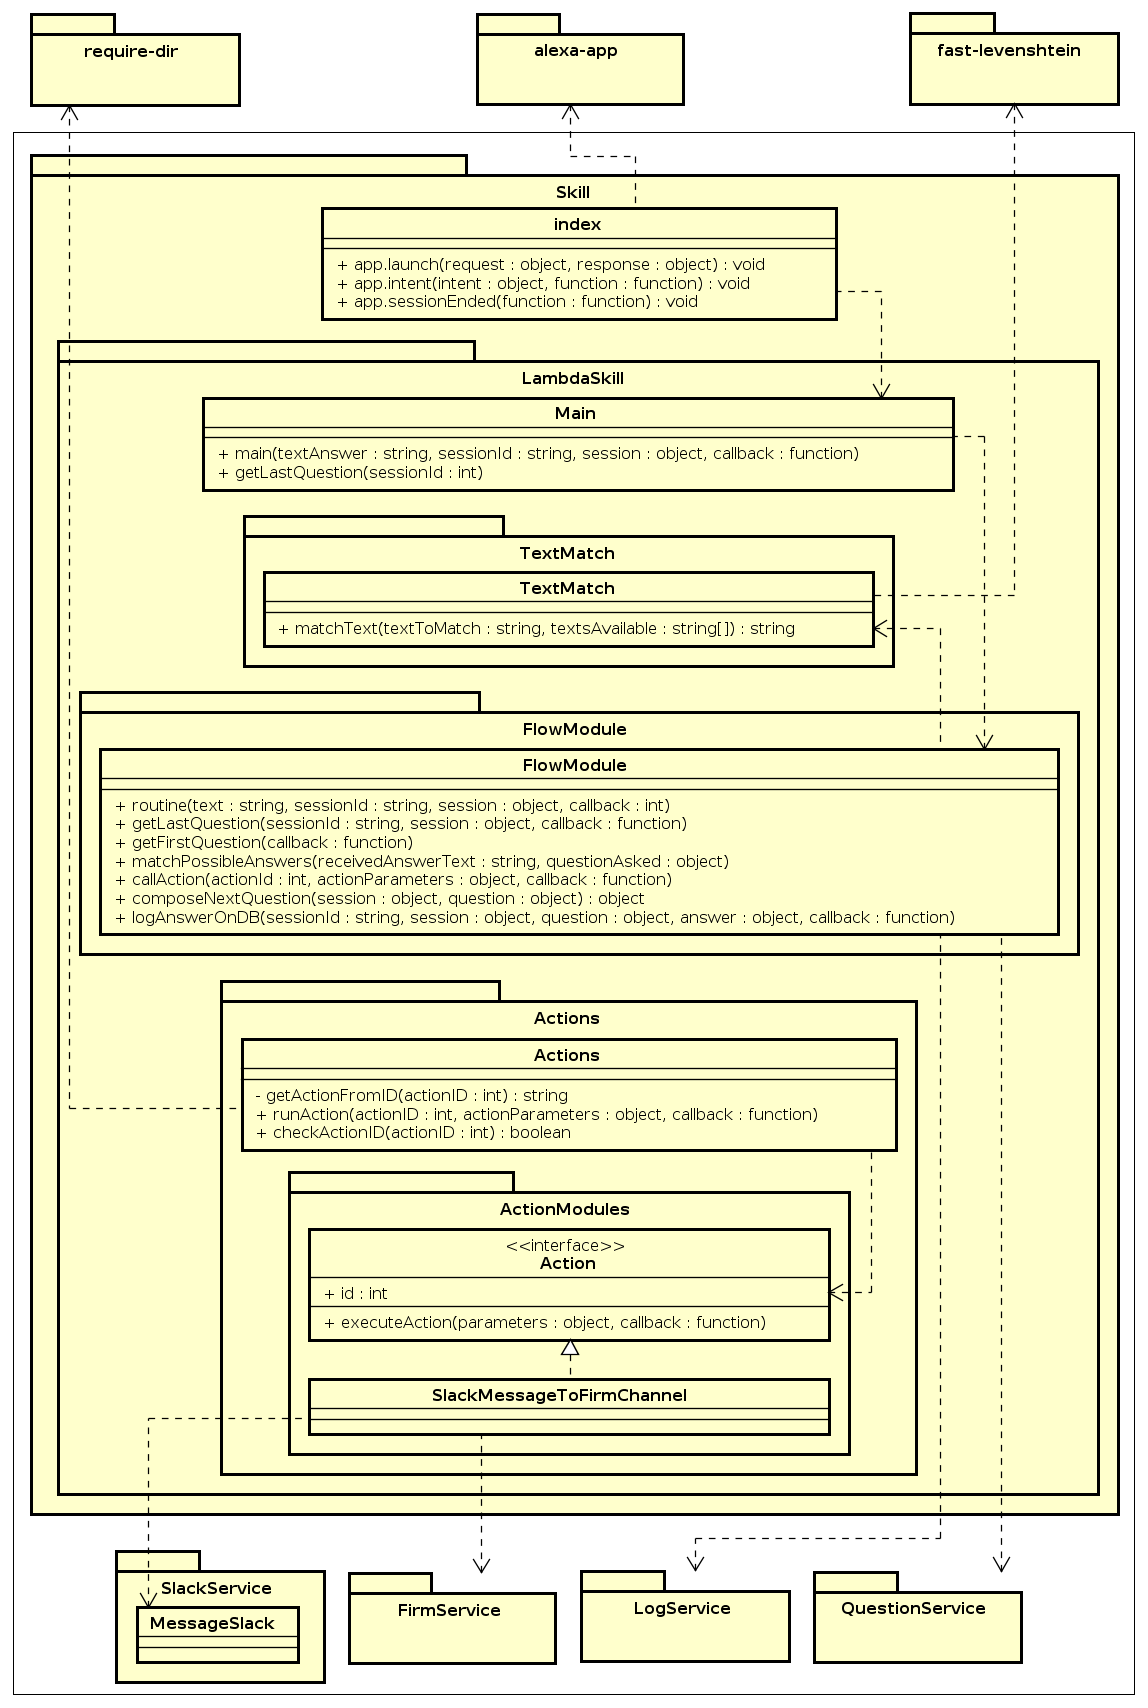
\includegraphics[scale=0.45]{Architettura/Back-End/Skill.png}
	\caption{Schema del componente \texttt{Front-End - Schema Generale}}
\end{figure}
\subparagraph{Descrizione}:
Package contenente la skill chiamata da Alexa tramite AVS.

\paragraph{\texttt{Back-End :: Skill :: index}}
\subparagraph{Descrizione}: Modulo per ottenere la lista degli utenti di Slack
\subparagraph{Dipendenze}:
\begin{itemize}
	\item \texttt{Back-End :: Skill :: LambdaSkill};
	\item \texttt{Alexa-app}.
\end{itemize}
\subparagraph{Metodi}:
\begin{itemize}
	\item \texttt{app.launch}
	      \subparagraph{Descrizione}: Handler per le chiamate alla Skill con intent Launch.
	      \subparagraph{Parametri}:
	      \begin{itemize}
	      	\item \texttt{callback}.
	      \end{itemize}
	      \subparagraph{Ritorno}: Utilizzando la callback, il metodo ottiene i dati della richiesta mandata da Alexa e crea l'oggetto risposta che verrà restituito in callback.
	\item \texttt{app.intent}
	      \subparagraph{Descrizione}: Handler per le chiamate alla Skill con intent custom.
	      \subparagraph{Parametri}:
	      \begin{itemize}
	      	\item \texttt{intentName};
	      	\item \texttt{intentConfiguration};
	      	\item \texttt{callback}.
	      \end{itemize}
	      \subparagraph{Ritorno}: Utilizzando la callback, il metodo ottiene i dati della richiesta mandata da Alexa e crea l'oggetto risposta che verrà restituito in callback.
	\item \texttt{app.sessionEnded}
	      \subparagraph{Descrizione}: Handler per le chiamate alla Skill con intent ended.
	      \subparagraph{Parametri}:
	      \begin{itemize}
	      	\item \texttt{callback}.
	      \end{itemize}
	      \subparagraph{Ritorno}: Utilizzando la callback, il metodo ottiene i dati della richiesta mandata da Alexa e crea l'oggetto risposta che verrà restituito in callback.
	\item \texttt{app.utterances}
	      \subparagraph{Descrizione}: Ridefinizione del metodo per la generazione delle utterances.
	      \subparagraph{Ritorno}: Il metodo ritorna una stringa di utterances espansa.
\end{itemize}

\subsubsection{\texttt{Back-End :: Skill :: LambdaSkill}}
\subparagraph{Descrizione}: Package contenente la parte logica per l'interazione con l'ospite. Gestisce la sequenza di domande e riceve ed elabora le risposte.

\paragraph{\texttt{Back-End :: Skill :: LambdaSkill :: Main}}
\subparagraph{Descrizione}: Modulo per la gestione della logica della skill.
\subparagraph{Dipendenze}:
\begin{itemize}
	\item \texttt{Back-End :: Skill :: LambdaSkill :: FlowModule :: FlowModule}
\end{itemize}
\subparagraph{Costanti}:
\begin{itemize}
	\item \texttt{askFirmNameQuestion};
	\item \texttt{askGuestNameQuestion}.
\end{itemize}
\subparagraph{Metodi}:
\begin{itemize}
	\item \texttt{main}
	      \subparagraph{Descrizione}: Metodo che gestisce la chiamata alla routine di azioni da eseguire quando l'AV riceve una risposta da parte di Alexa.
	      \subparagraph{Parametri}:
	      \begin{itemize}
	      	\item \texttt{textAnswer};
	      	\item \texttt{sessionId};
	      	\item \texttt{session};
	      	\item \texttt{callback}.
	      \end{itemize}
	      \subparagraph{Ritorno}: Il metodo restituisce in callback il testo della risposta dell'AV.
\end{itemize}

\subsubsection{\texttt{Back-End :: Skill :: LambdaSkill :: TextMatch}}
\subparagraph{Descrizione}: Package che contiene i moduli per il confronto tra la risposta data dall'utente con le risposte rese disponibili dagli amministratori.

\paragraph{\texttt{Back-End :: Skill :: LambdaSkill :: TextMatch :: TextMatch}}
\subparagraph{Descrizione}: Package che rende disponibili i metodi matching del testo di una risposta con un array di possibili testi.
\subparagraph{Dipendenze}: \begin{itemize}
\item \texttt{fast-levenshtein}
\end{itemize}
\subparagraph{Metodi}
\begin{itemize}
	\item \texttt{matchText}
	      \subparagraph{Descrizione}: Metodo per il match di una stringa di testo con un array di stringhe di testo
	      \subparagraph{Parametri}:
	      \begin{itemize}
	      	\item \texttt{textToMatch};
	      	\item \texttt{textsAvailable}.
	      \end{itemize}
	      \subparagraph{Ritorno}: Il metodo restituisce il testo più vicino o un errore se troppo distante dai testi disponibili.
\end{itemize}

\subsubsection{\texttt{Back-End :: Skill :: LambdaSkill :: FlowModule}}
\subparagraph{Descrizione}:
Package che contiene il modulo per la gestione logica delle domande.

\paragraph{\texttt{Back-End :: Skill :: LambdaSkill :: FlowModule :: FlowModule}}
\subparagraph{Descrizione}: Modulo per la gestione logica dell'AV. Si occupa di risposte dell'utente e di formulare le domande.
\subparagraph{Dipendenze}:
\begin{itemize}
	\item \texttt{Back-End :: Skill :: LambdaSkill :: TextMatch};
	\item \texttt{Back-End :: Skill :: LambdaSkill :: Actions};
	\item \texttt{Back-End :: Service :: QuestionService};
	\item \texttt{Back-End :: Service :: LogService}.
\end{itemize}
\subparagraph{Metodi}:
\begin{itemize}
	\item \texttt{routine}
	      \subparagraph{Descrizione}: Metodo per la l'esecuzione della sequenza di azioni per la comprensione di una risposta e la generazione della domanda seguente.
	      \subparagraph{Parametri}:
	      \begin{itemize}
	      	\item \texttt{textAnswer};
	      	\item \texttt{sessionId};
	      	\item \texttt{sessionAttributes};
	      	\item \texttt{callback}.
	      \end{itemize}
	      \subparagraph{Ritorno}: Il metodo restituisce tramite la callback un oggetto JSON con i dati sulla prossima domanda da porre o un errore.

	\item \texttt{getLastQuestion}
	      \subparagraph{Descrizione}: Metodo per ottenere la domanda successiva, salvata sul DB in base alla risposta passata.
	      \subparagraph{Parametri}:
	      \begin{itemize}
	      	\item \texttt{answer};
	      	\item \texttt{sessionAttributes};
	      	\item \texttt{callback}.
	      \end{itemize}
	      \subparagraph{Ritorno}: Il metodo restituisce tramite la callback un oggetto JSON contenente la prossima domanda, con le relative risposte associate, oppure un errore.

	\item \texttt{getFirstQuestion}
	      \subparagraph{Descrizione}: Metodo per ottenere la prima domanda da porre all'ospite.
	      \subparagraph{Parametri}:
	      \begin{itemize}
	      	\item \texttt{callback}.
	      \end{itemize}
	      \subparagraph{Ritorno}: Il metodo restituisce tramite la callback un oggetto JSON contenente la prima domanda, con le relative risposte associate, oppure un errore.

	\item \texttt{matchPossibleAnswers}
	      \subparagraph{Descrizione}: Metodo per confrontare la risposta rilevata da AVS con le risposte disponibili.
	      \subparagraph{Parametri}:
	      \begin{itemize}
	      	\item \texttt{receivedAnswerText};
	      	\item \texttt{questionAsked}.
	      \end{itemize}
	      \subparagraph{Ritorno}: Il metodo restituisce l'oggetto answer più vicino alla risposta ricevuta oppure un errore.

	\item \texttt{composeNextQuestion}
	      \subparagraph{Descrizione}: Metodo per gestire la chiamata a questionAction e generare il testo delle domande dell'AV durante la conversazione.
	      \subparagraph{Parametri}:
	      \begin{itemize}
	      	\item \texttt{sessionAttributes};
	      	\item \texttt{question};
			\item \texttt{callback}.
	      \end{itemize}
	      \subparagraph{Ritorno}: Il metodo restituisce in callback un oggetto JSON con la domanda o un errore.

	\item \texttt{callAction}
	      \subparagraph{Descrizione}: Metodo per lanciare l'esecuzione di una action.
	      \subparagraph{Parametri}:
	      \begin{itemize}
	      	\item \texttt{actionId};
	      	\item \texttt{actionParameters};
	      	\item \texttt{callback}.
	      \end{itemize}
	      \subparagraph{Ritorno}: Il metodo restituisce in callback il risultato dell'esecuzione dell'action o un errore.

	\item \texttt{callQuestionAction}
	      \subparagraph{Descrizione}: Metodo per lanciare l'esecuzione di una questionAction.
	      \subparagraph{Parametri}:
	      \begin{itemize}
	      	\item \texttt{questionActionId};
	      	\item \texttt{actionParameters};
	      	\item \texttt{callback}.
	      \end{itemize}
	      \subparagraph{Ritorno}: Il metodo restituisce in callback il risultato dell'esecuzione della questionAction o un errore.

	\item \texttt{logAnswerOnDB}
	      \subparagraph{Descrizione}: Metodo per eseguire il log dell'interazione con l'ospite
	      \subparagraph{Parametri}:
	      \begin{itemize}
	      	\item \texttt{sessionId};
	      	\item \texttt{sessionAttributes};
	      	\item \texttt{question};
	      	\item \texttt{answer};
	      	\item \texttt{callback}.
	      \end{itemize}
	      \subparagraph{Ritorno}: Il metodo restituisce in callback il risultato dell'esecuzione del log o un errore.

\end{itemize}

\subsubsection{\texttt{Back-End :: Skill :: LambdaSkill :: Actions}}
\subparagraph{Descrizione}: Package che contiene il modulo per l'esecuzione delle action.

\paragraph{\texttt{Back-End :: Skill :: LambdaSkill :: Actions :: Actions}}
\subparagraph{Descrizione}: Modulo per la gestione e la chiamata delle Actions
\subparagraph{Dipendenze}:
\begin{itemize}
	\item \texttt{require-dir};
	\item \texttt{Back-End :: Skill :: LambdaSkill :: Actions :: ActionsModules :: *}
\end{itemize}
\subparagraph{Metodi}:
\begin{itemize}
	\item \texttt{runAction}
	      \subparagraph{Descrizione}: Metodo per eseguire un action. Esegue l'action con id actionID passando i parametri actionParameters.
	      \subparagraph{Parametri}:
	      \begin{itemize}
	      	\item \texttt{actionID};
	      	\item \texttt{actionParameters};
	      	\item \texttt{callback}.
	      \end{itemize}
	      \subparagraph{Ritorno}: Il metodo esegue l'azione indicata e restituisce in callback il risultato dell'esecuzione.
	\item \texttt{checkActionID}
	      \subparagraph{Descrizione}: Metodo per la verifica della validità dell'actionID
	      \subparagraph{Parametri}:
	      \begin{itemize}
	      	\item \texttt{actionID}.
	      \end{itemize}
	      \subparagraph{Ritorno}: Il metodo restituisce true se l'actionID è legato ad un action in ActionModules; false altrimenti.
\end{itemize}

\subsubsection{\texttt{Back-End :: Skill :: LambdaSkill :: Actions :: ActionModules}}
\subparagraph{Descrizione}:
Package che contiene tutti i moduli delle action disponibili al sistema.

\paragraph{\texttt{Back-End :: Skill :: LambdaSkill :: Actions :: Actions :: SlackMessageToFirmChannel}}
\subparagraph{Descrizione}: Modulo action per inviare un messaggio ad un canale azienda Slack.
\subparagraph{Dipendenze}:
\begin{itemize}
	\item \texttt{Back-End :: Service :: MessageSlack}.
\end{itemize}
\subparagraph{Costanti}:
\begin{itemize}
	\item \texttt{id}.
\end{itemize}
\subparagraph{Metodi}:
\begin{itemize}
	\item \texttt{executeAction}.
	      \subparagraph{Descrizione}: Metodo di chiamata dell'action. Invia un messaggio ad un canale azienda Slack in base al contenuto del campo parameters.
	      \subparagraph{Parametri}:
	      \begin{itemize}
	      	\item \texttt{actionID};
	      	\item \texttt{actionParameters};
	      	\item \texttt{callback}.
	      \end{itemize}
	      \subparagraph{Ritorno}: Il metodo esegue l'azione indicata e restituisce in callback il risultato dell'esecuzione.
\end{itemize}

\subsection{\texttt{AVS}}
	\subparagraph{Descrizione}: Package che si riferisce al componente esterno AVS (Alexa Voice Service), il quale viene utilizzato all'interno dell'architettura

\subsection{\texttt{aws-sdk}}

	\subparagraph{Descrizione}: Package che si riferisce al componente esterno aws-sdk (Amazon Web Services SDK), il quale viene utilizzato all'interno dell'architettura

\end{document}
